% /* vim: set filetype=tex: */
\documentclass{article}
\usepackage{amsmath}
\usepackage{color}
\usepackage{fancyvrb}
\usepackage{framed}
\definecolor{shadecolor}{RGB}{240,240,240}
\usepackage{parskip}
\DefineVerbatimEnvironment{Highlighting}{Verbatim}{commandchars=\\\{\}}
% Add ',fontsize=\small' for more characters per line
\usepackage{framed}
\definecolor{shadecolor}{RGB}{248,248,248}
%\newenvironment{Shaded}{}{}
\newenvironment{Shaded}{\begin{snugshade}}{\end{snugshade}}
\newcommand{\KeywordTok}[1]{\textcolor[rgb]{0.00,0.44,0.13}{\textbf{#1}}}
\newcommand{\DataTypeTok}[1]{\textcolor[rgb]{0.56,0.13,0.00}{#1}}
\newcommand{\DecValTok}[1]{\textcolor[rgb]{0.25,0.63,0.44}{#1}}
\newcommand{\BaseNTok}[1]{\textcolor[rgb]{0.25,0.63,0.44}{#1}}
\newcommand{\FloatTok}[1]{\textcolor[rgb]{0.25,0.63,0.44}{#1}}
\newcommand{\ConstantTok}[1]{\textcolor[rgb]{0.53,0.00,0.00}{#1}}
\newcommand{\CharTok}[1]{\textcolor[rgb]{0.25,0.44,0.63}{#1}}
\newcommand{\SpecialCharTok}[1]{\textcolor[rgb]{0.25,0.44,0.63}{#1}}
\newcommand{\StringTok}[1]{\textcolor[rgb]{0.25,0.44,0.63}{#1}}
\newcommand{\VerbatimStringTok}[1]{\textcolor[rgb]{0.25,0.44,0.63}{#1}}
\newcommand{\SpecialStringTok}[1]{\textcolor[rgb]{0.73,0.40,0.53}{#1}}
%\newcommand{\ImportTok}[1]{#1}
\newcommand{\CommentTok}[1]{\textcolor[rgb]{0.38,0.63,0.69}{\textit{#1}}}
\newcommand{\DocumentationTok}[1]{\textcolor[rgb]{0.73,0.13,0.13}{\textit{#1}}}
\newcommand{\AnnotationTok}[1]{\textcolor[rgb]{0.38,0.63,0.69}{\textbf{\textit{#1}}}}
\newcommand{\CommentVarTok}[1]{\textcolor[rgb]{0.38,0.63,0.69}{\textbf{\textit{#1}}}}
\newcommand{\OtherTok}[1]{\textcolor[rgb]{0.00,0.44,0.13}{#1}}
\newcommand{\FunctionTok}[1]{\textcolor[rgb]{0.02,0.16,0.49}{#1}}
\newcommand{\VariableTok}[1]{\textcolor[rgb]{0.10,0.09,0.49}{#1}}
%\newcommand{\ControlFlowTok}[1]{\textcolor[rgb]{0.00,0.44,0.13}{\textbf{#1}}}
%\newcommand{\OperatorTok}[1]{\textcolor[rgb]{0.40,0.40,0.40}{#1}}
%\newcommand{\BuiltInTok}[1]{#1}
\newcommand{\ExtensionTok}[1]{#1}
\newcommand{\PreprocessorTok}[1]{\textcolor[rgb]{0.74,0.48,0.00}{#1}}
\newcommand{\AttributeTok}[1]{\textcolor[rgb]{0.49,0.56,0.16}{#1}}
\newcommand{\RegionMarkerTok}[1]{#1}
\newcommand{\InformationTok}[1]{\textcolor[rgb]{0.38,0.63,0.69}{\textbf{\textit{#1}}}}
\newcommand{\WarningTok}[1]{\textcolor[rgb]{0.38,0.63,0.69}{\textbf{\textit{#1}}}}
\newcommand{\AlertTok}[1]{\textcolor[rgb]{1.00,0.00,0.00}{\textbf{#1}}}
\newcommand{\ErrorTok}[1]{\textcolor[rgb]{1.00,0.00,0.00}{\textbf{#1}}}
\newcommand{\NormalTok}[1]{#1}

\setlength{\parindent}{0cm}
\usepackage[a4paper]{geometry}
\geometry{scale={0.80,0.85}}
\usepackage{booktabs}
\usepackage{longtable}
\usepackage{graphicx}
\setkeys{Gin}{width=.75\csname Gin@nat@width\endcsname,keepaspectratio}
\let\oldincludegraphics\includegraphics
\renewcommand\includegraphics[2][]{%
\begin{center}\oldincludegraphics[]{#2}\end{center}
}
\DeclareGraphicsExtensions{%
    .pdf,.PDF,%
    .png,.PNG,%
    .jpg,.mps,.jpeg,.jbig2,.jb2,.JPG,.JPEG,.JBIG2,.JB2}
\usepackage{floatrow}    
\renewcommand{\arraystretch}{1.2}
\usepackage{framed}

\usepackage[colorlinks=true,
linkcolor=blue]{hyperref}


\newcommand{\pkg}[1]{{\normalfont\fontseries{b}\selectfont #1}}
\let\proglang=\textsf
\let\code=\texttt

\title{The \textsf{lavaan} tutorial} 
\author{Yves Rosseel\\Department of Data Analysis\\%
  Ghent University (Belgium)}

\providecommand{\tightlist}{%
  \setlength{\itemsep}{0pt}\setlength{\parskip}{0pt}}

%\newcommand{\KeywordTok}[1]{\textcolor[rgb]{0.00,0.44,0.13}{\textbf{{#1}}}}
\newcommand{\BuiltInTok}[1]{\textcolor[rgb]{0.00,0.44,0.13}{\textbf{{#1}}}}
\newcommand{\OperatorTok}[1]{\textcolor[rgb]{0.00,0.44,0.13}{\textbf{{#1}}}}
\newcommand{\ControlFlowTok}[1]{\textcolor[rgb]{0.00,0.44,0.13}{\textbf{{#1}}}}
\newcommand{\ImportTok}[1]{\textcolor[rgb]{0.00,0.44,0.13}{\textbf{{#1}}}}
%\newcommand{\DataTypeTok}[1]{\textcolor[rgb]{0.56,0.13,0.00}{{#1}}}

\begin{document}
\maketitle
\begin{abstract}
If you are new to \pkg{lavaan}, this is the place to start. In this tutorial, we
introduce the basic components of lavaan: the model syntax, the fitting
functions (cfa, sem and growth), and the main extractor functions (summary,
coef, fitted, inspect). After we have provided two simple examples, we briefly
discuss some important topics: meanstructures, multiple groups, growth curve
models, mediation analysis, and categorical data. Along the way, we hope to
give you just enough information to get you started (but no more).
\end{abstract}

\tableofcontents

\section{Before you start}
Before you start, please read these points carefully:

\begin{itemize}
\item
  First of all, you must have a recent version (4.0.0 or higher) of R
  installed. You can download the latest version of R from this page:
  \url{http://cran.r-project.org/}.
\item
  Some important features are NOT available (yet) in lavaan:

  \begin{itemize}
  \item
    multilevel sem with random slopes (this is under developement)
  \item
    support for variable types other than continuous, binary and ordinal
    (for example: zero-inflated count data, nominal data, non-Gaussian
    continuous data); it is unlikely that this will be part of lavaan
    any time soon, for the simple reason that these variable types need
    numerical quadrature, and this is too slow to be practical in (pure)
    R.
  \item
    support for discrete latent variables (mixture models, latent
    classes) (although you can use the sampling weights and multiple
    group features to mimic some mixture models)
  \end{itemize}

  We hope to add these features to lavaan in the near future (but please
  do not ask when).
\item
  The lavaan package is free open-source software. This means (among
  other things) that there is no warranty whatsoever. On the other hand,
  you can verify the source code yourself:
  \url{https://github.com/yrosseel/lavaan/}
\item
  If you need help, you can (only) ask questions in the lavaan
  discussion group. Go to
  \url{https://groups.google.com/d/forum/lavaan/} and join the group.
  Once you have joined the group, you can email your questions to
  \href{mailto:lavaan@googlegroups.com}{\nolinkurl{lavaan@googlegroups.com}}.
  Please do not email me directly.
\item
  I do not offer statistical advice. For general (non lavaan-specific)
  questions about SEM, consider posting to the SEMNET discussion group.
\item
  If you think you have found a bug, or if you have a suggestion for
  improvement, you can either email me directly, or open an issue on
  github (see \url{https://github.com/yrosseel/lavaan/issues}). If you
  report a bug, always provide a minimal reproducible example (a short R
  script and some data).
\end{itemize}

\section{Installation of the package}
The lavaan package is available on CRAN. Therefore, to install lavaan,
simply start up R, and type in the R console:

\begin{Shaded}
\begin{Highlighting}[]
\FunctionTok{install.packages}\NormalTok{(}\StringTok{"lavaan"}\NormalTok{, }\AttributeTok{dependencies =} \ConstantTok{TRUE}\NormalTok{)}
\end{Highlighting}
\end{Shaded}

You can check if the installation was succesful by typing

\begin{Shaded}
\begin{Highlighting}[]
\FunctionTok{library}\NormalTok{(lavaan)}
\end{Highlighting}
\end{Shaded}

\begin{verbatim}
This is lavaan 0.6-11
lavaan is FREE software! Please report any bugs.
\end{verbatim}

A startup message will be displayed showing the version number (always
report this in your papers), and a reminder that this is free software.
If you see this message, you are ready to start.

\section{The model syntax}
At the heart of the lavaan package is the `model syntax'. The model
syntax is a description of the model to be estimated. In this section,
we briefly explain the elements of the lavaan model syntax. More details
are given in the examples that follow.

In the R environment, a regression formula has the following form:

\begin{verbatim}
y ~ x1 + x2 + x3 + x4
\end{verbatim}

In this formula, the tilde (``\texttt{\textasciitilde{}}'') is the
regression operator. On the left-hand side of the operator, we have the
dependent variable (\texttt{y}), and on the right-hand side, we have the
independent variables, separated by the ``\texttt{+}'' operator. In
lavaan, a typical model is simply a set (or system) of regression
formulas, where some variables (starting with an `\texttt{f}' below) may
be latent. For example:

\begin{verbatim}
 y ~ f1 + f2 + x1 + x2 
f1 ~ f2 + f3 
f2 ~ f3 + x1 + x2
\end{verbatim}

If we have latent variables in any of the regression formulas, we must
`define' them by listing their (manifest or latent) indicators. We do
this by using the special operator ``\texttt{=\textasciitilde{}}'',
which can be read as \emph{is measured by}. For example, to define the
three latent variabels \texttt{f1}, \texttt{f2} and \texttt{f3}, we can
use something like:

\begin{verbatim}
f1 =~ y1 + y2 + y3 
f2 =~ y4 + y5 + y6 
f3 =~ y7 + y8 + y9 + y10
\end{verbatim}

Furthermore, variances and covariances are specified using a `double
tilde' operator, for example:

\begin{verbatim}
y1 ~~ y1  # variance
y1 ~~ y2  # covariance
f1 ~~ f2  # covariance
\end{verbatim}

And finally, intercepts for observed and latent variables are simple
regression formulas with only an intercept (explicitly denoted by the
number `\texttt{1}') as the only predictor:

\begin{verbatim}
y1 ~ 1
f1 ~ 1
\end{verbatim}

Using these four \emph{formula types}, a large variety of latent
variable models can be described. The current set of formula types is
summarized in the table below.

\begin{longtable}[]{@{}lll@{}}
\toprule
formula type & operator & mnemonic\tabularnewline
\midrule
\endhead
latent variable definition & \texttt{=\textasciitilde{}} & is measured
by\tabularnewline
regression & \texttt{\textasciitilde{}} & is regressed on\tabularnewline
(residual) (co)variance & \texttt{\textasciitilde{}\textasciitilde{}} &
is correlated with\tabularnewline
intercept & \texttt{\textasciitilde{}\ 1} & intercept\tabularnewline
\bottomrule
\end{longtable}

A complete lavaan model syntax is simply a combination of these formula
types, enclosed between \emph{single} quotes. For example:

\begin{Shaded}
\begin{Highlighting}[]
\NormalTok{myModel <-}\StringTok{ ' # regressions}
\StringTok{             y1 + y2 ~ f1 + f2 + x1 + x2}
\StringTok{                  f1 ~ f2 + f3}
\StringTok{                  f2 ~ f3 + x1 + x2}

\StringTok{             # latent variable definitions }
\StringTok{               f1 =~ y1 + y2 + y3 }
\StringTok{               f2 =~ y4 + y5 + y6 }
\StringTok{               f3 =~ y7 + y8 + y9 + y10}

\StringTok{             # variances and covariances }
\StringTok{               y1 ~~ y1 }
\StringTok{               y1 ~~ y2 }
\StringTok{               f1 ~~ f2}

\StringTok{             # intercepts }
\StringTok{               y1 ~ 1 }
\StringTok{               f1 ~ 1}
\StringTok{           '}
\end{Highlighting}
\end{Shaded}

You can type this syntax interactively at the R prompt, but it is much
more convenient to type the whole model syntax first in an external text
editor. And when you are done, you can copy/paste it to the R console.
If you are using \href{http://www.rstudio.com/}{RStudio}, open a new `R
script', and type your model syntax (and all other R commands needed for
this session) in the source editor of RStudio. And save your script, so
you can reuse it later on.

The code piece above will produce a model syntax object, called
\texttt{myModel} that can be used later when calling a function that
actually estimates this model given a dataset. Note that formulas can be
split over multiple lines, and you can use comments (starting with the
\texttt{\#} character) and blank lines within the single quotes to
improve the readability of the model syntax.

If your model syntax is rather long, or you need to reuse the model
syntax over and over again, you may prefer to store it in a separate
text file called, say, \texttt{myModel.lav}. This text file should be in
a human readable format (not a Word document). Within R, you can then
read the model syntax from the file as follows:

\begin{Shaded}
\begin{Highlighting}[]
\NormalTok{    myModel <-}\StringTok{ }\KeywordTok{readLines}\NormalTok{(}\StringTok{"/mydirectory/myModel.lav"}\NormalTok{)}
\end{Highlighting}
\end{Shaded}

The argument of \texttt{readLines} is the full path to the file
containing the model syntax. Again, the model syntax object can be used
later to fit this model given a dataset.

\section{A first example: confirmatory factor analysis (CFA)}
We start with a simple example of confirmatory factor analysis, using
the \texttt{cfa()} function, which is a user-friendly function for
fitting CFA models. The lavaan package contains a built-in dataset
called \texttt{HolzingerSwineford1939}. See the help page for this
dataset by typing

\begin{verbatim}
?HolzingerSwineford1939
\end{verbatim}

at the R prompt. This is a `classic' dataset that is used in many papers
and books on Structural Equation Modeling (SEM), including some manuals
of commercial SEM software packages. The data consists of mental ability
test scores of seventh- and eighth-grade children from two different
schools (Pasteur and Grant-White). In our version of the dataset, only 9
out of the original 26 tests are included. A CFA model that is often
proposed for these 9 variables consists of three latent variables (or
factors), each with three indicators:

\begin{itemize}
\tightlist
\item
  a \emph{visual} factor measured by 3 variables: \texttt{x1},
  \texttt{x2} and \texttt{x3}
\item
  a \emph{textual} factor measured by 3 variables: \texttt{x4},
  \texttt{x5} and \texttt{x6}
\item
  a \emph{speed} factor measured by 3 variables: \texttt{x7},
  \texttt{x8} and \texttt{x9}
\end{itemize}

The figure below contains a graphical representation of the three-factor
model.

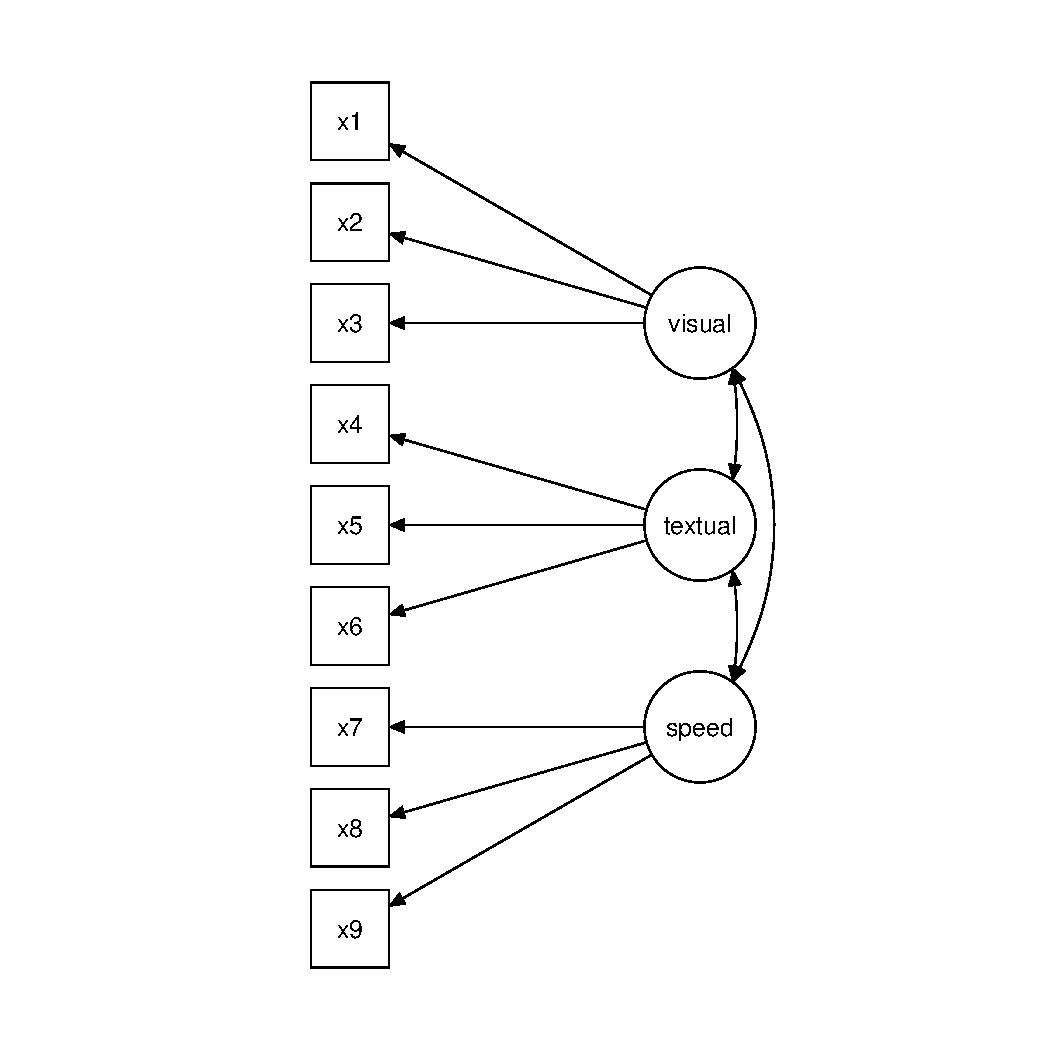
\includegraphics{figure/cfa-1.pdf} The corresponding lavaan syntax for
specifying this model is as follows:

\begin{verbatim}
 visual =~ x1 + x2 + x3
textual =~ x4 + x5 + x6
  speed =~ x7 + x8 + x9
\end{verbatim}

In this example, the model syntax only contains three `latent variable
definitions'. Each formula has the following format:

\begin{verbatim}
latent variable =~ indicator1 + indicator2 + indicator3
\end{verbatim}

We call these expressions \emph{latent variable definitions} because
they define how the latent variables are `manifested by' a set of
observed (or manifest) variables, often called `indicators'. Note that
the special ``\texttt{=\textasciitilde{}"} operator in the middle
consists of a sign (''\texttt{=}``) character and a tilde
(\texttt{"\textasciitilde{}"}) character next to each other. The reason
why this model syntax is so short, is that behind the scenes, the
function will take care of several things. First, by default, the factor
loading of the first indicator of a latent variable is fixed to 1,
thereby fixing the scale of the latent variable. Second, residual
variances are added automatically. And third, all exogenous latent
variables are correlated by default. This way, the model syntax can be
kept concise. On the other hand, the user remains in control, since all
this `default' behavior can be overriden and/or switched off.

We can enter the model syntax using the single quotes:

\begin{Shaded}
\begin{Highlighting}[]
\NormalTok{HS.model <-}\StringTok{ ' visual  =~ x1 + x2 + x3 }
\StringTok{              textual =~ x4 + x5 + x6}
\StringTok{              speed   =~ x7 + x8 + x9 '}
\end{Highlighting}
\end{Shaded}

We can now fit the model as follows:

\begin{Shaded}
\begin{Highlighting}[]
\NormalTok{fit <-}\StringTok{ }\KeywordTok{cfa}\NormalTok{(HS.model, }\DataTypeTok{data=}\NormalTok{HolzingerSwineford1939)}
\end{Highlighting}
\end{Shaded}

The \texttt{cfa()} function is a dedicated function for fitting
confirmatory factor analysis models. The first argument is the
user-specified model. The second argument is the dataset that contains
the observed variables. Once the model has been fitted, the
\texttt{summary()} function provides a nice summary of the fitted model:

\begin{Shaded}
\begin{Highlighting}[]
\KeywordTok{summary}\NormalTok{(fit, }\DataTypeTok{fit.measures=}\OtherTok{TRUE}\NormalTok{)}
\end{Highlighting}
\end{Shaded}

The output should look familiar to users of other SEM software. If you
find it confusing or esthetically unpleasing, please let us know, and we
will try to improve it.

\begin{verbatim}
lavaan (0.6-1) converged normally after  35 iterations

  Number of observations                           301

  Estimator                                         ML
  Model Fit Test Statistic                      85.306
  Degrees of freedom                                24
  P-value (Chi-square)                           0.000

Model test baseline model:

  Minimum Function Test Statistic              918.852
  Degrees of freedom                                36
  P-value                                        0.000

User model versus baseline model:

  Comparative Fit Index (CFI)                    0.931
  Tucker-Lewis Index (TLI)                       0.896

Loglikelihood and Information Criteria:

  Loglikelihood user model (H0)              -3737.745
  Loglikelihood unrestricted model (H1)      -3695.092

  Number of free parameters                         21
  Akaike (AIC)                                7517.490
  Bayesian (BIC)                              7595.339
  Sample-size adjusted Bayesian (BIC)         7528.739

Root Mean Square Error of Approximation:

  RMSEA                                          0.092
  90 Percent Confidence Interval          0.071  0.114
  P-value RMSEA <= 0.05                          0.001

Standardized Root Mean Square Residual:

  SRMR                                           0.065

Parameter Estimates:

  Information                                 Expected
  Information saturated (h1) model          Structured
  Standard Errors                             Standard

Latent Variables:
                   Estimate  Std.Err  z-value  P(>|z|)
  visual =~                                           
    x1                1.000                           
    x2                0.554    0.100    5.554    0.000
    x3                0.729    0.109    6.685    0.000
  textual =~                                          
    x4                1.000                           
    x5                1.113    0.065   17.014    0.000
    x6                0.926    0.055   16.703    0.000
  speed =~                                            
    x7                1.000                           
    x8                1.180    0.165    7.152    0.000
    x9                1.082    0.151    7.155    0.000

Covariances:
                   Estimate  Std.Err  z-value  P(>|z|)
  visual ~~                                           
    textual           0.408    0.074    5.552    0.000
    speed             0.262    0.056    4.660    0.000
  textual ~~                                          
    speed             0.173    0.049    3.518    0.000

Variances:
                   Estimate  Std.Err  z-value  P(>|z|)
   .x1                0.549    0.114    4.833    0.000
   .x2                1.134    0.102   11.146    0.000
   .x3                0.844    0.091    9.317    0.000
   .x4                0.371    0.048    7.779    0.000
   .x5                0.446    0.058    7.642    0.000
   .x6                0.356    0.043    8.277    0.000
   .x7                0.799    0.081    9.823    0.000
   .x8                0.488    0.074    6.573    0.000
   .x9                0.566    0.071    8.003    0.000
    visual            0.809    0.145    5.564    0.000
    textual           0.979    0.112    8.737    0.000
    speed             0.384    0.086    4.451    0.000
\end{verbatim}

The output consists of three parts. The first six lines are called
\emph{the header}. The header contains the following information:

\begin{itemize}
\tightlist
\item
  the lavaan version number
\item
  did lavaan converge normally or not, and how many iterations were
  needed
\item
  the number of observations that were effectively used in the analysis
\item
  the estimator that was used to obtain the parameter values (here:
  \texttt{ML})
\item
  the model test statistic, the degrees of freedom, and a corresponding
  p-value
\end{itemize}

The next section contains additional fit measures, and is only shown
because we use the optional argument \texttt{fit.measures\ =\ TRUE}. It
starts with the line \texttt{Model\ test\ baseline\ model} and ends with
the value for the \texttt{SRMR}. The last section contains the parameter
estimates. It starts with information about the standard errors (if the
information matrix is expected or observed, and if the standard errors
are standard, robust, or based on the bootstrap). Then, it tabulates all
free (and fixed) parameters that were included in the model. Typically,
first the latent variables are shown, followed by covariances and
(residual) variances. The first column (\texttt{Estimate}) contains the
(estimated or fixed) parameter value for each model parameter; the
second column (\texttt{Std.err}) contains the standard error for each
estimated parameter; the third column (\texttt{Z-value}) contains the
Wald statistic (which is simply obtained by dividing the parameter value
by its standard error), and the last column
(\texttt{P(\textgreater{}\textbar{}z\textbar{})}) contains the p-value
for testing the null hypothesis that the parameter equals zero in the
population.

To wrap up this first example, we summarize the complete code that was
needed to fit this three-factor model:

\begin{Shaded}
\begin{Highlighting}[]
\CommentTok{# load the lavaan package (only needed once per session)}
\KeywordTok{library}\NormalTok{(lavaan)}

\CommentTok{# specify the model}
\NormalTok{HS.model <-}\StringTok{ ' visual  =~ x1 + x2 + x3      }
\StringTok{              textual =~ x4 + x5 + x6}
\StringTok{              speed   =~ x7 + x8 + x9 '}

\CommentTok{# fit the model}
\NormalTok{fit <-}\StringTok{ }\KeywordTok{cfa}\NormalTok{(HS.model, }\DataTypeTok{data=}\NormalTok{HolzingerSwineford1939)}

\CommentTok{# display summary output}
\KeywordTok{summary}\NormalTok{(fit, }\DataTypeTok{fit.measures=}\OtherTok{TRUE}\NormalTok{)}
\end{Highlighting}
\end{Shaded}

Simply copying this code and pasting it in R should work. The syntax
illustrates the typical workflow in the lavaan package:

\begin{enumerate}
\def\labelenumi{\arabic{enumi}.}
\item
  Specify your model using the lavaan model syntax. In this example,
  only \emph{latent variable definitions} have been used. In the
  following examples, other formula types will be used.
\item
  Fit the model. This requires a dataset containing the observed
  variables (or alternatively the sample covariance matrix and the
  number of observations). In this example, we have used the
  \texttt{cfa()} function. Other funcions in the lavaan package are
  \texttt{sem()} and \texttt{growth()} for fitting full structural
  equation models and growth curve models respectively. All three
  functions are so-called user-friendly functions, in the sense that
  they take care of many details automatically, so we can keep the model
  syntax simple and concise. If you wish to fit non-standard models or
  if you don't like the idea that things are done for you automatically,
  you can use the lower-level function \texttt{lavaan()} instead, where
  you have full control.
\item
  Extract information from the fitted model. This can be a long verbose
  summary, or it can be a single number only (say, the RMSEA value). In
  the spirit of R, you only get what you asked for. We try to not print
  out unnecessary information that you would ignore anyway.
\end{enumerate}

\section{A second example: a structural equation model (SEM)}
In our second example, we will use the built-in
\texttt{PoliticalDemocracy} dataset. This is a dataset that has been
used by Bollen in his 1989 book on structural equation modeling (and
elsewhere). To learn more about the dataset, see its help page and the
references therein.

The figure below contains a graphical representation of the model that
we want to fit.

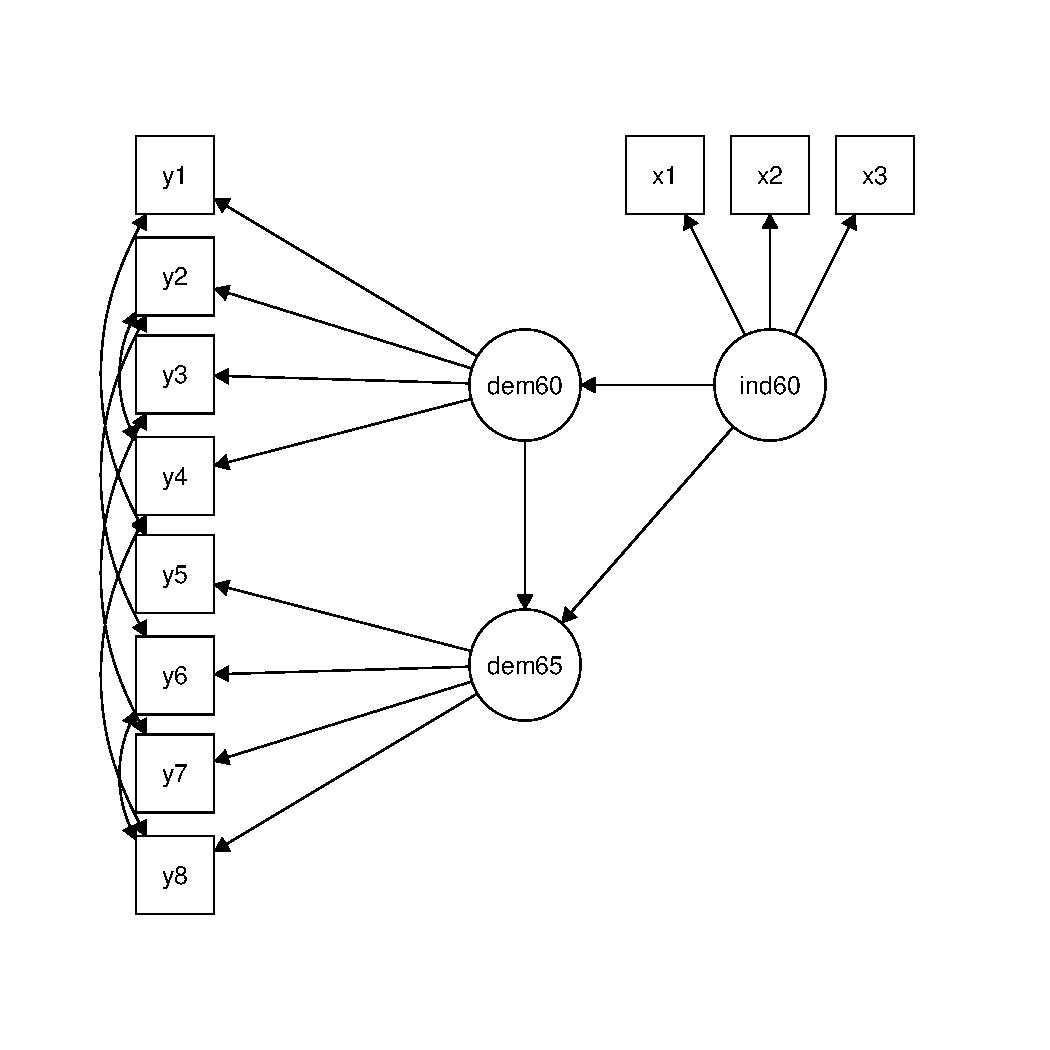
\includegraphics{figure/sem-1.pdf}

The corresponding lavaan syntax for specifying this model is as follows:

\begin{Shaded}
\begin{Highlighting}[]
\NormalTok{model }\OtherTok{\textless{}{-}} \StringTok{\textquotesingle{}}
\StringTok{  \# measurement model}
\StringTok{    ind60 =\textasciitilde{} x1 + x2 + x3}
\StringTok{    dem60 =\textasciitilde{} y1 + y2 + y3 + y4}
\StringTok{    dem65 =\textasciitilde{} y5 + y6 + y7 + y8}
\StringTok{  \# regressions}
\StringTok{    dem60 \textasciitilde{} ind60}
\StringTok{    dem65 \textasciitilde{} ind60 + dem60}
\StringTok{  \# residual correlations}
\StringTok{    y1 \textasciitilde{}\textasciitilde{} y5}
\StringTok{    y2 \textasciitilde{}\textasciitilde{} y4 + y6}
\StringTok{    y3 \textasciitilde{}\textasciitilde{} y7}
\StringTok{    y4 \textasciitilde{}\textasciitilde{} y8}
\StringTok{    y6 \textasciitilde{}\textasciitilde{} y8}
\StringTok{\textquotesingle{}}
\end{Highlighting}
\end{Shaded}

In this example, we use three different formula types: latent variabele
definitions (using the \texttt{=\textasciitilde{}} operator), regression
formulas (using the \texttt{\textasciitilde{}} operator), and
(co)variance formulas (using the
\texttt{\textasciitilde{}\textasciitilde{}} operator). The regression
formulas are similar to ordinary formulas in R. The (co)variance
formulas typically have the following form:

\begin{verbatim}
variable ~~ variable
\end{verbatim}

The variables can be either observed or latent variables. If the two
variable names are the same, the expression refers to the variance (or
residual variance) of that variable. If the two variable names are
different, the expression refers to the (residual) covariance among
these two variables. The lavaan package automatically makes the
distinction between variances and residual variances.

In our example, the expression
\texttt{y1\ \textasciitilde{}\textasciitilde{}\ y5} allows the residual
variances of the two observed variables to be correlated. This is
sometimes done if it is believed that the two variables have something
in common that is not captured by the latent variables. In this case,
the two variables refer to identical scores, but measured in two
different years (1960 and 1965, respectively). Note that the two
expressions \texttt{y2\ \textasciitilde{}\textasciitilde{}\ y4} and
\texttt{y2\ \textasciitilde{}\textasciitilde{}\ y6}, can be combined
into the expression
\texttt{y2\ \textasciitilde{}\textasciitilde{}~y4\ +\ y6}, because the
variable on the left of the \texttt{\textasciitilde{}\textasciitilde{}}
operator (\texttt{y2}) is the same. This is just a shorthand notation.

We enter the model syntax as follows:

\begin{Shaded}
\begin{Highlighting}[]
\NormalTok{model }\OtherTok{\textless{}{-}} \StringTok{\textquotesingle{}}
\StringTok{  \# measurement model}
\StringTok{    ind60 =\textasciitilde{} x1 + x2 + x3}
\StringTok{    dem60 =\textasciitilde{} y1 + y2 + y3 + y4}
\StringTok{    dem65 =\textasciitilde{} y5 + y6 + y7 + y8}
\StringTok{  \# regressions}
\StringTok{    dem60 \textasciitilde{} ind60}
\StringTok{    dem65 \textasciitilde{} ind60 + dem60}
\StringTok{  \# residual correlations}
\StringTok{    y1 \textasciitilde{}\textasciitilde{} y5}
\StringTok{    y2 \textasciitilde{}\textasciitilde{} y4 + y6}
\StringTok{    y3 \textasciitilde{}\textasciitilde{} y7}
\StringTok{    y4 \textasciitilde{}\textasciitilde{} y8}
\StringTok{    y6 \textasciitilde{}\textasciitilde{} y8}
\StringTok{\textquotesingle{}}
\end{Highlighting}
\end{Shaded}

To fit the model and see the results we can type:

\begin{Shaded}
\begin{Highlighting}[]
\NormalTok{fit }\OtherTok{\textless{}{-}} \FunctionTok{sem}\NormalTok{(model, }\AttributeTok{data =}\NormalTok{ PoliticalDemocracy)}
\FunctionTok{summary}\NormalTok{(fit, }\AttributeTok{standardized =} \ConstantTok{TRUE}\NormalTok{)}
\end{Highlighting}
\end{Shaded}

\begin{verbatim}
lavaan 0.6-11 ended normally after 68 iterations

  Estimator                                         ML
  Optimization method                           NLMINB
  Number of model parameters                        31
                                                      
  Number of observations                            75
                                                      
Model Test User Model:
                                                      
  Test statistic                                38.125
  Degrees of freedom                                35
  P-value (Chi-square)                           0.329

Parameter Estimates:

  Standard errors                             Standard
  Information                                 Expected
  Information saturated (h1) model          Structured

Latent Variables:
                   Estimate  Std.Err  z-value  P(>|z|)   Std.lv  Std.all
  ind60 =~                                                              
    x1                1.000                               0.670    0.920
    x2                2.180    0.139   15.742    0.000    1.460    0.973
    x3                1.819    0.152   11.967    0.000    1.218    0.872
  dem60 =~                                                              
    y1                1.000                               2.223    0.850
    y2                1.257    0.182    6.889    0.000    2.794    0.717
    y3                1.058    0.151    6.987    0.000    2.351    0.722
    y4                1.265    0.145    8.722    0.000    2.812    0.846
  dem65 =~                                                              
    y5                1.000                               2.103    0.808
    y6                1.186    0.169    7.024    0.000    2.493    0.746
    y7                1.280    0.160    8.002    0.000    2.691    0.824
    y8                1.266    0.158    8.007    0.000    2.662    0.828

Regressions:
                   Estimate  Std.Err  z-value  P(>|z|)   Std.lv  Std.all
  dem60 ~                                                               
    ind60             1.483    0.399    3.715    0.000    0.447    0.447
  dem65 ~                                                               
    ind60             0.572    0.221    2.586    0.010    0.182    0.182
    dem60             0.837    0.098    8.514    0.000    0.885    0.885

Covariances:
                   Estimate  Std.Err  z-value  P(>|z|)   Std.lv  Std.all
 .y1 ~~                                                                 
   .y5                0.624    0.358    1.741    0.082    0.624    0.296
 .y2 ~~                                                                 
   .y4                1.313    0.702    1.871    0.061    1.313    0.273
   .y6                2.153    0.734    2.934    0.003    2.153    0.356
 .y3 ~~                                                                 
   .y7                0.795    0.608    1.308    0.191    0.795    0.191
 .y4 ~~                                                                 
   .y8                0.348    0.442    0.787    0.431    0.348    0.109
 .y6 ~~                                                                 
   .y8                1.356    0.568    2.386    0.017    1.356    0.338

Variances:
                   Estimate  Std.Err  z-value  P(>|z|)   Std.lv  Std.all
   .x1                0.082    0.019    4.184    0.000    0.082    0.154
   .x2                0.120    0.070    1.718    0.086    0.120    0.053
   .x3                0.467    0.090    5.177    0.000    0.467    0.239
   .y1                1.891    0.444    4.256    0.000    1.891    0.277
   .y2                7.373    1.374    5.366    0.000    7.373    0.486
   .y3                5.067    0.952    5.324    0.000    5.067    0.478
   .y4                3.148    0.739    4.261    0.000    3.148    0.285
   .y5                2.351    0.480    4.895    0.000    2.351    0.347
   .y6                4.954    0.914    5.419    0.000    4.954    0.443
   .y7                3.431    0.713    4.814    0.000    3.431    0.322
   .y8                3.254    0.695    4.685    0.000    3.254    0.315
    ind60             0.448    0.087    5.173    0.000    1.000    1.000
   .dem60             3.956    0.921    4.295    0.000    0.800    0.800
   .dem65             0.172    0.215    0.803    0.422    0.039    0.039
\end{verbatim}

The function \texttt{sem()} is very similar to the function
\texttt{cfa()}. In fact, the two functions are currently almost
identical, but this may change in the future. In the \texttt{summary()}
function, we omitted the \texttt{fit.measures\ =\ TRUE} argument.
Therefore, you only get the basic chi-square test statistic. The
argument \texttt{standardized\ =\ TRUE} augments the output with
standardized parameter values. Two extra columns of standardized
parameter values are printed. In the first column (labeled
\texttt{Std.lv}), only the latent variables are standardized. In the
second column (labeled \texttt{Std.all}), both latent and observed
variables are standardized. The latter is often called the `completely
standardized solution'.

The complete code to specify and fit this model is printed again below:

\begin{Shaded}
\begin{Highlighting}[]
\FunctionTok{library}\NormalTok{(lavaan) }\CommentTok{\# only needed once per session}
\NormalTok{model }\OtherTok{\textless{}{-}} \StringTok{\textquotesingle{}}
\StringTok{  \# measurement model}
\StringTok{    ind60 =\textasciitilde{} x1 + x2 + x3}
\StringTok{    dem60 =\textasciitilde{} y1 + y2 + y3 + y4}
\StringTok{    dem65 =\textasciitilde{} y5 + y6 + y7 + y8}
\StringTok{  \# regressions}
\StringTok{    dem60 \textasciitilde{} ind60}
\StringTok{    dem65 \textasciitilde{} ind60 + dem60}
\StringTok{  \# residual correlations}
\StringTok{    y1 \textasciitilde{}\textasciitilde{} y5}
\StringTok{    y2 \textasciitilde{}\textasciitilde{} y4 + y6}
\StringTok{    y3 \textasciitilde{}\textasciitilde{} y7}
\StringTok{    y4 \textasciitilde{}\textasciitilde{} y8}
\StringTok{    y6 \textasciitilde{}\textasciitilde{} y8}
\StringTok{\textquotesingle{}}
\NormalTok{fit }\OtherTok{\textless{}{-}} \FunctionTok{sem}\NormalTok{(model, }\AttributeTok{data=}\NormalTok{PoliticalDemocracy)}
\FunctionTok{summary}\NormalTok{(fit, }\AttributeTok{standardized=}\ConstantTok{TRUE}\NormalTok{)}
\end{Highlighting}
\end{Shaded}

\section{More about the syntax}
\hypertarget{fixing-parameters}{%
\paragraph{Fixing parameters}\label{fixing-parameters}}

Consider a simple one-factor model with 4 indicators. By default, lavaan
will always fix the factor loading of the first indicator to 1. The
other three factor loadings are free, and their values are estimated by
the model. But suppose that you have good reasons to fix all the factor
loadings to 1. The syntax below illustrates how this can be done:

\begin{verbatim}
f =~ y1 + 1*y2 + 1*y3 + 1*y4
\end{verbatim}

In general, to fix a parameter in a lavaan formula, you need to
pre-multiply the corresponding variable in the formula by a numerical
value. This is called the pre-multiplication mechanism and will be used
for many purposes. As another example, consider again the three-factor
Holzinger and Swineford CFA model. Recall that, by default, all
exogenous latent variables in a CFA model are correlated. But if you
wish to fix the correlation (or covariance) between a pair of latent
variables to zero, you need to explicity add a covariance-formula for
this pair, and fix the parameter to zero. In the syntax below, we allow
the covariance between the latent variables \texttt{visual} and
\texttt{textual} to be free, but the two other covariances are fixed to
zero. In addition, we fix the variance of the factor \texttt{speed} to
unity. Therefore, there is no need anymore to set the factor loading of
its first indicator (\texttt{x7}) equal to one. To force this factor
loading to be free, we pre-multiply it with \texttt{NA}, as a hint to
lavaan that the value of this parameter is `missing' and therefore still
unknown.

\begin{verbatim}
# three-factor model
   visual =~ x1 + x2 + x3
  textual =~ x4 + x5 + x6
  speed   =~ NA*x7 + x8 + x9
# orthogonal factors
   visual ~~ 0*speed
  textual ~~ 0*speed
# fix variance of speed factor
    speed ~~ 1*speed
\end{verbatim}

If you need to constrain all covariances of the latent variables in a
CFA model to be orthogonal, there is a shortcut. You can omit the
covariance formulas in the model syntax and simply add an argument
\texttt{orthogonal\ =\ TRUE} to the function call:

\begin{Shaded}
\begin{Highlighting}[]
\NormalTok{HS.model }\OtherTok{\textless{}{-}} \StringTok{\textquotesingle{} visual  =\textasciitilde{} x1 + x2 + x3}
\StringTok{              textual =\textasciitilde{} x4 + x5 + x6}
\StringTok{              speed   =\textasciitilde{} x7 + x8 + x9 \textquotesingle{}}

\NormalTok{fit.HS.ortho }\OtherTok{\textless{}{-}} \FunctionTok{cfa}\NormalTok{(HS.model, }
                    \AttributeTok{data =}\NormalTok{ HolzingerSwineford1939, }
                    \AttributeTok{orthogonal =} \ConstantTok{TRUE}\NormalTok{)}
\end{Highlighting}
\end{Shaded}

Similarly, if you want to fix the variances of \emph{all} the latent
variables in a CFA model to unity, there is again a shortcut. Simply add
the argument \texttt{std.lv\ =\ TRUE} to the function call:

\begin{Shaded}
\begin{Highlighting}[]
\NormalTok{HS.model }\OtherTok{\textless{}{-}} \StringTok{\textquotesingle{} visual  =\textasciitilde{} x1 + x2 + x3}
\StringTok{              textual =\textasciitilde{} x4 + x5 + x6}
\StringTok{              speed   =\textasciitilde{} x7 + x8 + x9 \textquotesingle{}}

\NormalTok{fit }\OtherTok{\textless{}{-}} \FunctionTok{cfa}\NormalTok{(HS.model, }
           \AttributeTok{data =}\NormalTok{ HolzingerSwineford1939, }
           \AttributeTok{std.lv =} \ConstantTok{TRUE}\NormalTok{)}
\end{Highlighting}
\end{Shaded}

If the argument \texttt{std.lv\ =\ TRUE} is used, the factor loadings of
the first indicator of each latent variable will no longer be fixed to
1.

\hypertarget{starting-values}{%
\paragraph{Starting Values}\label{starting-values}}

The lavaan package automatically generates starting values for all free
parameters. Normally, this works fine. But if you prefer to provide your
own starting values, you are free to do so. The way it works is based on
the pre-multiplication mechanism that we discussed before. But the
numeric constant is now the argument of a special function
\texttt{start()}. An example will make this clear:

\begin{verbatim}
visual  =~ x1 + start(0.8)*x2 + start(1.2)*x3
textual =~ x4 + start(0.5)*x5 + start(1.0)*x6
speed   =~ x7 + start(0.7)*x8 + start(1.8)*x9
\end{verbatim}

\hypertarget{parameter-labels}{%
\paragraph{Parameter labels}\label{parameter-labels}}

A nice property of the lavaan package is that all free parameters are
automatically named according to a simple set of rules. This is
convenient, for example, if equality constraints are needed (see the
next subsection). To see how the naming mechanism works, we will use the
model that we used for the Politcal Democracy data.

\begin{Shaded}
\begin{Highlighting}[]
\NormalTok{model }\OtherTok{\textless{}{-}} \StringTok{\textquotesingle{}}
\StringTok{  \# latent variable definitions}
\StringTok{    ind60 =\textasciitilde{} x1 + x2 + x3}
\StringTok{    dem60 =\textasciitilde{} y1 + y2 + y3 + y4}
\StringTok{    dem65 =\textasciitilde{} y5 + y6 + y7 + y8}
\StringTok{  \# regressions}
\StringTok{    dem60 \textasciitilde{} ind60}
\StringTok{    dem65 \textasciitilde{} ind60 + dem60}
\StringTok{  \# residual (co)variances}
\StringTok{    y1 \textasciitilde{}\textasciitilde{} y5}
\StringTok{    y2 \textasciitilde{}\textasciitilde{} y4 + y6}
\StringTok{    y3 \textasciitilde{}\textasciitilde{} y7}
\StringTok{    y4 \textasciitilde{}\textasciitilde{} y8}
\StringTok{    y6 \textasciitilde{}\textasciitilde{} y8}
\StringTok{\textquotesingle{}}

\NormalTok{fit }\OtherTok{\textless{}{-}} \FunctionTok{sem}\NormalTok{(model, }
           \AttributeTok{data =}\NormalTok{ PoliticalDemocracy)}

\FunctionTok{coef}\NormalTok{(fit)}
\end{Highlighting}
\end{Shaded}

\begin{verbatim}
   ind60=~x2    ind60=~x3    dem60=~y2    dem60=~y3    dem60=~y4    dem65=~y6 
       2.180        1.819        1.257        1.058        1.265        1.186 
   dem65=~y7    dem65=~y8  dem60~ind60  dem65~ind60  dem65~dem60       y1~~y5 
       1.280        1.266        1.483        0.572        0.837        0.624 
      y2~~y4       y2~~y6       y3~~y7       y4~~y8       y6~~y8       x1~~x1 
       1.313        2.153        0.795        0.348        1.356        0.082 
      x2~~x2       x3~~x3       y1~~y1       y2~~y2       y3~~y3       y4~~y4 
       0.120        0.467        1.891        7.373        5.067        3.148 
      y5~~y5       y6~~y6       y7~~y7       y8~~y8 ind60~~ind60 dem60~~dem60 
       2.351        4.954        3.431        3.254        0.448        3.956 
dem65~~dem65 
       0.172 
\end{verbatim}

The function \texttt{coef()} extracts the estimated values of the free
parameters in the model, together with their names. Each name consists
of three parts and reflects the part of the formula where the parameter
was involved. The first part is the variable name that appears on the
left-hand side (lhs) of the formula. The middle part is the operator
type (op) of the formula, and the third part is the variable in the
right-hand side (rhs) of the formula that corresponds with the
parameter.

Often, it is convenient to choose your own labels for specific
parameters. The way this works is similar to fixing a parameter. But
instead of pre-multiplying with a numerical constant, we use a character
string (the label) instead. In the example below, we `label' the factor
loading of the \texttt{x3} indicator with the label \texttt{myLabel}:

\begin{Shaded}
\begin{Highlighting}[]
\NormalTok{model }\OtherTok{\textless{}{-}} \StringTok{\textquotesingle{}}
\StringTok{  \# latent variable definitions}
\StringTok{    ind60 =\textasciitilde{} x1 + x2 + myLabel*x3}
\StringTok{    dem60 =\textasciitilde{} y1 + y2 + y3 + y4}
\StringTok{    dem65 =\textasciitilde{} y5 + y6 + y7 + y8}
\StringTok{  \# regressions}
\StringTok{    dem60 \textasciitilde{} ind60}
\StringTok{    dem65 \textasciitilde{} ind60 + dem60}
\StringTok{  \# residual (co)variances}
\StringTok{    y1 \textasciitilde{}\textasciitilde{} y5}
\StringTok{    y2 \textasciitilde{}\textasciitilde{} y4 + y6}
\StringTok{    y3 \textasciitilde{}\textasciitilde{} y7}
\StringTok{    y4 \textasciitilde{}\textasciitilde{} y8}
\StringTok{    y6 \textasciitilde{}\textasciitilde{} y8}
\StringTok{\textquotesingle{}}
\end{Highlighting}
\end{Shaded}

It is important that labels start with a letter (a-zA-Z), and certainly
not with a digit. For example `13bis' is not a valid label, and will
confuse the lavaan syntax parser. (Note: before version 0.4-8, it was
necessary to use the modifier \texttt{label()} to specify a custom
label. Although it is still supported, it is not recommended anymore.
The only reason why it should be used in new syntax is if the label
contains an operator like ``\texttt{=\textasciitilde{}}''.)

\hypertarget{modifiers}{%
\paragraph{Modifiers}\label{modifiers}}

We have seen the use of the pre-multiplication mechanism (using the
\texttt{*} operator) a number of times: to fix a parameter, to provide a
starting value, and to label a parameter. We refer to these operations
as \emph{modifiers}, because they modify some properties of certain
model parameters. More modifiers will be introduced later.

Each term on the right hand side in a formula can have one modifier
only. If you want to specify more modifiers for the same parameter, you
need to list the term multiple times in the same formula. For example:

\begin{verbatim}
f =~ y1 + y2 + myLabel*y3 + start(0.5)*y3 + y4
\end{verbatim}

The indicator \texttt{y3} was listed twice, each time with a different
modifier. The parser will accumulate all the different modifiers, but
still treat \texttt{y3} as a single indicator.

\hypertarget{simple-equality-constraints}{%
\paragraph{Simple equality
constraints}\label{simple-equality-constraints}}

In some applications, it is useful to impose equality constraints on one
or more otherwise free parameters. Consider again the three-factor H\&S
CFA model. Suppose a user has a priori reasons to believe that the
factor loadings of the \texttt{x2} and \texttt{x3} indicators are equal
to each other. Instead of estimating two free parameters, lavaan should
only estimate a single free parameter, and use that value for both
factor loadings. The main mechanism to specify this type of (simple)
equality constraints is by using labels: if two parameters have the same
label, they will be considered to be the same, and only one value will
be computed for them. This is illustrated in the following syntax:

\begin{verbatim}
visual  =~ x1 + v2*x2 + v2*x3
textual =~ x4 + x5 + x6
speed   =~ x7 + x8 + x9
\end{verbatim}

Remember: all parameters having the same label will be constrained to be
equal.

An alternative approach is to use the \texttt{equal()} modifier. This is
useful if no custom label has been specified, and one needs to refer to
the automatically generated label. For example:

\begin{verbatim}
visual  =~ x1 + x2 + equal("visual=~x2")*x3
textual =~ x4 + x5 + x6
speed   =~ x7 + x8 + x9
\end{verbatim}

\hypertarget{nonlinear-equality-and-inequality-constraints}{%
\paragraph{Nonlinear equality and inequality
constraints}\label{nonlinear-equality-and-inequality-constraints}}

Consider the following regression:

\begin{verbatim}
y ~ b1*x1 + b2*x2 + b3*x3
\end{verbatim}

where we have explicitly labeled the regression coefficients as
\texttt{b1}, \texttt{b2} and \texttt{b3}. We create a toy dataset
containing these four variables and fit the regression model:

\begin{Shaded}
\begin{Highlighting}[]
\FunctionTok{set.seed}\NormalTok{(}\DecValTok{1234}\NormalTok{)}
\NormalTok{Data }\OtherTok{\textless{}{-}} \FunctionTok{data.frame}\NormalTok{(}\AttributeTok{y  =} \FunctionTok{rnorm}\NormalTok{(}\DecValTok{100}\NormalTok{), }
                   \AttributeTok{x1 =} \FunctionTok{rnorm}\NormalTok{(}\DecValTok{100}\NormalTok{), }
                   \AttributeTok{x2 =} \FunctionTok{rnorm}\NormalTok{(}\DecValTok{100}\NormalTok{),}
                   \AttributeTok{x3 =} \FunctionTok{rnorm}\NormalTok{(}\DecValTok{100}\NormalTok{))}
\NormalTok{model }\OtherTok{\textless{}{-}} \StringTok{\textquotesingle{} y \textasciitilde{} b1*x1 + b2*x2 + b3*x3 \textquotesingle{}}
\NormalTok{fit }\OtherTok{\textless{}{-}} \FunctionTok{sem}\NormalTok{(model, }\AttributeTok{data =}\NormalTok{ Data)}
\FunctionTok{coef}\NormalTok{(fit)}
\end{Highlighting}
\end{Shaded}

\begin{verbatim}
    b1     b2     b3   y~~y 
-0.052  0.084  0.139  0.970 
\end{verbatim}

Suppose that we need to impose the following two (nonlinear) constraints
on \(b_1\): \(b_1 = (b_2+b_3)^2\) and \(b_1 \geq \exp(b_2 + b_3)\). The
first constraint is an equality constraint. The second is an inequality
constraint. To specify these constraints, you can use the following
syntax:

\begin{Shaded}
\begin{Highlighting}[]
\NormalTok{model.constr }\OtherTok{\textless{}{-}} \StringTok{\textquotesingle{} \# model with labeled parameters}
\StringTok{                    y \textasciitilde{} b1*x1 + b2*x2 + b3*x3}
\StringTok{                  \# constraints}
\StringTok{                    b1 == (b2 + b3)\^{}2}
\StringTok{                    b1 \textgreater{} exp(b2 + b3) \textquotesingle{}}
\end{Highlighting}
\end{Shaded}

To see the effect of the constraints, we refit the model:

\begin{Shaded}
\begin{Highlighting}[]
\NormalTok{model.constr }\OtherTok{\textless{}{-}} \StringTok{\textquotesingle{} \# model with labeled parameters}
\StringTok{                    y \textasciitilde{} b1*x1 + b2*x2 + b3*x3}
\StringTok{                  \# constraints}
\StringTok{                    b1 == (b2 + b3)\^{}2}
\StringTok{                    b1 \textgreater{} exp(b2 + b3) \textquotesingle{}}
\NormalTok{fit }\OtherTok{\textless{}{-}} \FunctionTok{sem}\NormalTok{(model.constr, }\AttributeTok{data =}\NormalTok{ Data)}
\FunctionTok{coef}\NormalTok{(fit)}
\end{Highlighting}
\end{Shaded}

\begin{verbatim}
    b1     b2     b3   y~~y 
 0.495 -0.405 -0.299  1.610 
\end{verbatim}

The reader can verify that the constraints are indeed respected. The
equality constraint holds exactly. The inequality constraint has
resulted in an equality between the left-hand side (\(b_1\)) and the
right-hand side (\(\exp(b_2 + b_3)\)).

\section{Bringing in the means}
By and large, structural equation models are used to model the
covariance matrix of the observed variables in a dataset. But in some
applications, it is useful to bring in the means of the observed
variables too. One way to do this is to explicitly refer to intercepts
in the lavaan syntax. This can be done by including `intercept formulas'
in the model syntax. An intercept formula has the following form:

\begin{verbatim}
variable ~ 1
\end{verbatim}

The left part of the expression contains the name of the observed or
latent variable. The right part contains the number \texttt{1},
representing the intercept. For example, in the three-factor H\&S CFA
model, we can add the intercepts of the observed variables as follows:

\begin{verbatim}
# three-factor model
  visual  =~ x1 + x2 + x3
  textual =~ x4 + x5 + x6
  speed   =~ x7 + x8 + x9
# intercepts
  x1 ~ 1
  x2 ~ 1
  x3 ~ 1
  x4 ~ 1
  x5 ~ 1
  x6 ~ 1
  x7 ~ 1
  x8 ~ 1
  x9 ~ 1
\end{verbatim}

However, it is more convenient to omit the intercept formulas in the
model syntax (unless you want to fix their values), and to add the
argument \texttt{meanstructure\ =\ TRUE} in the fitting function. For
example, we can refit the three-factor H\&S CFA model as follows:

\begin{Shaded}
\begin{Highlighting}[]
\NormalTok{fit }\OtherTok{\textless{}{-}} \FunctionTok{cfa}\NormalTok{(HS.model, }
           \AttributeTok{data =}\NormalTok{ HolzingerSwineford1939, }
           \AttributeTok{meanstructure =} \ConstantTok{TRUE}\NormalTok{)}
\FunctionTok{summary}\NormalTok{(fit) }
\end{Highlighting}
\end{Shaded}

\begin{verbatim}
lavaan 0.6-11 ended normally after 35 iterations

  Estimator                                         ML
  Optimization method                           NLMINB
  Number of model parameters                        30
                                                      
  Number of observations                           301
                                                      
Model Test User Model:
                                                      
  Test statistic                                85.306
  Degrees of freedom                                24
  P-value (Chi-square)                           0.000

Parameter Estimates:

  Standard errors                             Standard
  Information                                 Expected
  Information saturated (h1) model          Structured

Latent Variables:
                   Estimate  Std.Err  z-value  P(>|z|)
  visual =~                                           
    x1                1.000                           
    x2                0.554    0.100    5.554    0.000
    x3                0.729    0.109    6.685    0.000
  textual =~                                          
    x4                1.000                           
    x5                1.113    0.065   17.014    0.000
    x6                0.926    0.055   16.703    0.000
  speed =~                                            
    x7                1.000                           
    x8                1.180    0.165    7.152    0.000
    x9                1.082    0.151    7.155    0.000

Covariances:
                   Estimate  Std.Err  z-value  P(>|z|)
  visual ~~                                           
    textual           0.408    0.074    5.552    0.000
    speed             0.262    0.056    4.660    0.000
  textual ~~                                          
    speed             0.173    0.049    3.518    0.000

Intercepts:
                   Estimate  Std.Err  z-value  P(>|z|)
   .x1                4.936    0.067   73.473    0.000
   .x2                6.088    0.068   89.855    0.000
   .x3                2.250    0.065   34.579    0.000
   .x4                3.061    0.067   45.694    0.000
   .x5                4.341    0.074   58.452    0.000
   .x6                2.186    0.063   34.667    0.000
   .x7                4.186    0.063   66.766    0.000
   .x8                5.527    0.058   94.854    0.000
   .x9                5.374    0.058   92.546    0.000
    visual            0.000                           
    textual           0.000                           
    speed             0.000                           

Variances:
                   Estimate  Std.Err  z-value  P(>|z|)
   .x1                0.549    0.114    4.833    0.000
   .x2                1.134    0.102   11.146    0.000
   .x3                0.844    0.091    9.317    0.000
   .x4                0.371    0.048    7.779    0.000
   .x5                0.446    0.058    7.642    0.000
   .x6                0.356    0.043    8.277    0.000
   .x7                0.799    0.081    9.823    0.000
   .x8                0.488    0.074    6.573    0.000
   .x9                0.566    0.071    8.003    0.000
    visual            0.809    0.145    5.564    0.000
    textual           0.979    0.112    8.737    0.000
    speed             0.384    0.086    4.451    0.000
\end{verbatim}

As you can see in the output, the model includes intercept parameters
for both the observed and latent variables. By default, the
\texttt{cfa()} and \texttt{sem()} functions fix the latent variable
intercepts (which in this case correspond to the latent \emph{means}) to
zero. Otherwise, the model would not be estimable. Note that the
chi-square statistic and the number of degrees of freedom is the same as
in the original model (without a mean structure). The reason is that we
brought in some new data (a mean value for each of the 9 observed
variables), but we also added 9 additional parameters to the model (an
intercept for each of the 9 observed variables). The end result is an
identical fit. In practice, the only reason why a user would add
intercept-formulas in the model syntax, is because some constraints must
be specified on them. For example, suppose that we wish to fix the
intercepts of the variables \texttt{x1}, \texttt{x2}, \texttt{x3} and
\texttt{x4} to, say, 0.5. We would write the model syntax as follows:

\begin{verbatim}
# three-factor model
  visual  =~ x1 + x2 + x3
  textual =~ x4 + x5 + x6
  speed   =~ x7 + x8 + x9
# intercepts with fixed values
  x1 + x2 + x3 + x4 ~ 0.5*1
\end{verbatim}

where we have used the left-hand side of the formula to `repeat' the
right-hand side for each element of the left-hand side.

\section{Multiple groups}
The lavaan package has full support for multiple groups. To request a
multiple group analysis, you need to add the name of the group variable
in your dataset to the argument \texttt{group} in the fitting function.
By default, the same model is fitted in all groups. In the following
example, we fit the H\&S CFA model for the two schools (Pasteur and
Grant-White).

\begin{Shaded}
\begin{Highlighting}[]
\NormalTok{HS.model }\OtherTok{\textless{}{-}} \StringTok{\textquotesingle{} visual  =\textasciitilde{} x1 + x2 + x3}
\StringTok{              textual =\textasciitilde{} x4 + x5 + x6}
\StringTok{              speed   =\textasciitilde{} x7 + x8 + x9 \textquotesingle{}}

\NormalTok{fit }\OtherTok{\textless{}{-}} \FunctionTok{cfa}\NormalTok{(HS.model, }
           \AttributeTok{data =}\NormalTok{ HolzingerSwineford1939, }
           \AttributeTok{group =} \StringTok{"school"}\NormalTok{)}

\FunctionTok{summary}\NormalTok{(fit)}
\end{Highlighting}
\end{Shaded}

\begin{verbatim}
lavaan 0.6-11 ended normally after 57 iterations

  Estimator                                         ML
  Optimization method                           NLMINB
  Number of model parameters                        60
                                                      
  Number of observations per group:                   
    Pasteur                                        156
    Grant-White                                    145
                                                      
Model Test User Model:
                                                      
  Test statistic                               115.851
  Degrees of freedom                                48
  P-value (Chi-square)                           0.000
  Test statistic for each group:
    Pasteur                                     64.309
    Grant-White                                 51.542

Parameter Estimates:

  Standard errors                             Standard
  Information                                 Expected
  Information saturated (h1) model          Structured


Group 1 [Pasteur]:

Latent Variables:
                   Estimate  Std.Err  z-value  P(>|z|)
  visual =~                                           
    x1                1.000                           
    x2                0.394    0.122    3.220    0.001
    x3                0.570    0.140    4.076    0.000
  textual =~                                          
    x4                1.000                           
    x5                1.183    0.102   11.613    0.000
    x6                0.875    0.077   11.421    0.000
  speed =~                                            
    x7                1.000                           
    x8                1.125    0.277    4.057    0.000
    x9                0.922    0.225    4.104    0.000

Covariances:
                   Estimate  Std.Err  z-value  P(>|z|)
  visual ~~                                           
    textual           0.479    0.106    4.531    0.000
    speed             0.185    0.077    2.397    0.017
  textual ~~                                          
    speed             0.182    0.069    2.628    0.009

Intercepts:
                   Estimate  Std.Err  z-value  P(>|z|)
   .x1                4.941    0.095   52.249    0.000
   .x2                5.984    0.098   60.949    0.000
   .x3                2.487    0.093   26.778    0.000
   .x4                2.823    0.092   30.689    0.000
   .x5                3.995    0.105   38.183    0.000
   .x6                1.922    0.079   24.321    0.000
   .x7                4.432    0.087   51.181    0.000
   .x8                5.563    0.078   71.214    0.000
   .x9                5.418    0.079   68.440    0.000
    visual            0.000                           
    textual           0.000                           
    speed             0.000                           

Variances:
                   Estimate  Std.Err  z-value  P(>|z|)
   .x1                0.298    0.232    1.286    0.198
   .x2                1.334    0.158    8.464    0.000
   .x3                0.989    0.136    7.271    0.000
   .x4                0.425    0.069    6.138    0.000
   .x5                0.456    0.086    5.292    0.000
   .x6                0.290    0.050    5.780    0.000
   .x7                0.820    0.125    6.580    0.000
   .x8                0.510    0.116    4.406    0.000
   .x9                0.680    0.104    6.516    0.000
    visual            1.097    0.276    3.967    0.000
    textual           0.894    0.150    5.963    0.000
    speed             0.350    0.126    2.778    0.005


Group 2 [Grant-White]:

Latent Variables:
                   Estimate  Std.Err  z-value  P(>|z|)
  visual =~                                           
    x1                1.000                           
    x2                0.736    0.155    4.760    0.000
    x3                0.925    0.166    5.583    0.000
  textual =~                                          
    x4                1.000                           
    x5                0.990    0.087   11.418    0.000
    x6                0.963    0.085   11.377    0.000
  speed =~                                            
    x7                1.000                           
    x8                1.226    0.187    6.569    0.000
    x9                1.058    0.165    6.429    0.000

Covariances:
                   Estimate  Std.Err  z-value  P(>|z|)
  visual ~~                                           
    textual           0.408    0.098    4.153    0.000
    speed             0.276    0.076    3.639    0.000
  textual ~~                                          
    speed             0.222    0.073    3.022    0.003

Intercepts:
                   Estimate  Std.Err  z-value  P(>|z|)
   .x1                4.930    0.095   51.696    0.000
   .x2                6.200    0.092   67.416    0.000
   .x3                1.996    0.086   23.195    0.000
   .x4                3.317    0.093   35.625    0.000
   .x5                4.712    0.096   48.986    0.000
   .x6                2.469    0.094   26.277    0.000
   .x7                3.921    0.086   45.819    0.000
   .x8                5.488    0.087   63.174    0.000
   .x9                5.327    0.085   62.571    0.000
    visual            0.000                           
    textual           0.000                           
    speed             0.000                           

Variances:
                   Estimate  Std.Err  z-value  P(>|z|)
   .x1                0.715    0.126    5.676    0.000
   .x2                0.899    0.123    7.339    0.000
   .x3                0.557    0.103    5.409    0.000
   .x4                0.315    0.065    4.870    0.000
   .x5                0.419    0.072    5.812    0.000
   .x6                0.406    0.069    5.880    0.000
   .x7                0.600    0.091    6.584    0.000
   .x8                0.401    0.094    4.249    0.000
   .x9                0.535    0.089    6.010    0.000
    visual            0.604    0.160    3.762    0.000
    textual           0.942    0.152    6.177    0.000
    speed             0.461    0.118    3.910    0.000
\end{verbatim}

If you want to fix parameters, or provide starting values, you can use
the same pre-multiplication techniques, but the single argument is now
replaced by a \emph{vector} of arguments, one for each group. If you use
a single element instead of a vector (which is not recommended), that
element will be applied for all groups. If you specify a single label,
this will generate a warning as this would imply equality constraints
across groups. For example:

\begin{Shaded}
\begin{Highlighting}[]
\NormalTok{HS.model }\OtherTok{\textless{}{-}} \StringTok{\textquotesingle{} visual  =\textasciitilde{} x1 + 0.5*x2 + c(0.6, 0.8)*x3}
\StringTok{              textual =\textasciitilde{} x4 + start(c(1.2, 0.6))*x5 + c(a1, a2)*x6}
\StringTok{              speed   =\textasciitilde{} x7 + x8 + x9 \textquotesingle{}}
\end{Highlighting}
\end{Shaded}

In the definition of the latent factor \texttt{visual}, we have fixed
the factor loading of the indicator \texttt{x3} to the value `0.6' in
the first group, and to the value `0.8' in the second group, while the
factor loading of the indicator \texttt{x2} is fixed to the value `0.5'
in both groups. In the definition of the \texttt{textual} factor, two
different starting values are provided for the \texttt{x5} indicator;
one for each group. In addition, we have labeled the factor loading of
the \texttt{x6} indicator as \texttt{a1} in the first group, and
\texttt{a2} in the second group. It may be tempting to write
\texttt{a*x6}. But using a single label in a multiple group setting has
a double effect: it gives the label \texttt{a} to the factor loading of
\texttt{x6} in both groups, and as a result, those two parameters are
now constrained to be equal. Because this may unintended, lavaan will
produce a warning message about this. If this is really intended, it is
much better to use a vector of labels: \texttt{c(a,\ a)*x6}.

To verify the effects of our modifiers, we refit the model:

\begin{Shaded}
\begin{Highlighting}[]
\NormalTok{fit }\OtherTok{\textless{}{-}} \FunctionTok{cfa}\NormalTok{(HS.model, }
           \AttributeTok{data =}\NormalTok{ HolzingerSwineford1939, }
           \AttributeTok{group =} \StringTok{"school"}\NormalTok{)}
 \FunctionTok{summary}\NormalTok{(fit)}
\end{Highlighting}
\end{Shaded}

\begin{verbatim}
lavaan 0.6-11 ended normally after 45 iterations

  Estimator                                         ML
  Optimization method                           NLMINB
  Number of model parameters                        56
                                                      
  Number of observations per group:                   
    Pasteur                                        156
    Grant-White                                    145
                                                      
Model Test User Model:
                                                      
  Test statistic                               118.976
  Degrees of freedom                                52
  P-value (Chi-square)                           0.000
  Test statistic for each group:
    Pasteur                                     64.901
    Grant-White                                 54.075

Parameter Estimates:

  Standard errors                             Standard
  Information                                 Expected
  Information saturated (h1) model          Structured


Group 1 [Pasteur]:

Latent Variables:
                   Estimate  Std.Err  z-value  P(>|z|)
  visual =~                                           
    x1                1.000                           
    x2                0.500                           
    x3                0.600                           
  textual =~                                          
    x4                1.000                           
    x5                1.185    0.102   11.598    0.000
    x6        (a1)    0.876    0.077   11.409    0.000
  speed =~                                            
    x7                1.000                           
    x8                1.129    0.279    4.055    0.000
    x9                0.931    0.227    4.103    0.000

Covariances:
                   Estimate  Std.Err  z-value  P(>|z|)
  visual ~~                                           
    textual           0.460    0.103    4.479    0.000
    speed             0.182    0.076    2.408    0.016
  textual ~~                                          
    speed             0.181    0.069    2.625    0.009

Intercepts:
                   Estimate  Std.Err  z-value  P(>|z|)
   .x1                4.941    0.094   52.379    0.000
   .x2                5.984    0.100   59.945    0.000
   .x3                2.487    0.092   26.983    0.000
   .x4                2.823    0.092   30.689    0.000
   .x5                3.995    0.105   38.183    0.000
   .x6                1.922    0.079   24.320    0.000
   .x7                4.432    0.087   51.181    0.000
   .x8                5.563    0.078   71.214    0.000
   .x9                5.418    0.079   68.440    0.000
    visual            0.000                           
    textual           0.000                           
    speed             0.000                           

Variances:
                   Estimate  Std.Err  z-value  P(>|z|)
   .x1                0.388    0.129    3.005    0.003
   .x2                1.304    0.155    8.432    0.000
   .x3                0.965    0.120    8.016    0.000
   .x4                0.427    0.069    6.153    0.000
   .x5                0.454    0.086    5.270    0.000
   .x6                0.289    0.050    5.763    0.000
   .x7                0.824    0.124    6.617    0.000
   .x8                0.510    0.116    4.417    0.000
   .x9                0.677    0.105    6.479    0.000
    visual            1.001    0.172    5.803    0.000
    textual           0.892    0.150    5.953    0.000
    speed             0.346    0.125    2.768    0.006


Group 2 [Grant-White]:

Latent Variables:
                   Estimate  Std.Err  z-value  P(>|z|)
  visual =~                                           
    x1                1.000                           
    x2                0.500                           
    x3                0.800                           
  textual =~                                          
    x4                1.000                           
    x5                0.990    0.087   11.425    0.000
    x6        (a2)    0.963    0.085   11.374    0.000
  speed =~                                            
    x7                1.000                           
    x8                1.228    0.188    6.539    0.000
    x9                1.081    0.168    6.417    0.000

Covariances:
                   Estimate  Std.Err  z-value  P(>|z|)
  visual ~~                                           
    textual           0.454    0.099    4.585    0.000
    speed             0.315    0.079    4.004    0.000
  textual ~~                                          
    speed             0.222    0.073    3.049    0.002

Intercepts:
                   Estimate  Std.Err  z-value  P(>|z|)
   .x1                4.930    0.097   50.688    0.000
   .x2                6.200    0.089   69.616    0.000
   .x3                1.996    0.086   23.223    0.000
   .x4                3.317    0.093   35.625    0.000
   .x5                4.712    0.096   48.986    0.000
   .x6                2.469    0.094   26.277    0.000
   .x7                3.921    0.086   45.819    0.000
   .x8                5.488    0.087   63.174    0.000
   .x9                5.327    0.085   62.571    0.000
    visual            0.000                           
    textual           0.000                           
    speed             0.000                           

Variances:
                   Estimate  Std.Err  z-value  P(>|z|)
   .x1                0.637    0.115    5.539    0.000
   .x2                0.966    0.120    8.076    0.000
   .x3                0.601    0.091    6.591    0.000
   .x4                0.316    0.065    4.877    0.000
   .x5                0.418    0.072    5.805    0.000
   .x6                0.407    0.069    5.887    0.000
   .x7                0.609    0.091    6.658    0.000
   .x8                0.411    0.094    4.385    0.000
   .x9                0.522    0.089    5.887    0.000
    visual            0.735    0.132    5.544    0.000
    textual           0.942    0.152    6.177    0.000
    speed             0.453    0.117    3.871    0.000
\end{verbatim}

\hypertarget{fixing-parameters-in-some-groups-but-not-all}{%
\paragraph{Fixing parameters in some groups, but not
all}\label{fixing-parameters-in-some-groups-but-not-all}}

Sometimes, we wish to fix the value of a parameter in all groups, except
for one particular group. In this group, we wish to freely estimate the
value of that parameter. The modifier for this parameter is again a
vector containing the fixed values for this parameter for each group,
but we can use \texttt{NA} to force a parameter to be free in one (or
more) group(s). Suppose for example we have four groups. We define a
latent variable (say \texttt{f}) with three indicators. We wish to fix
the factor loading of indicator \texttt{item2} to 1.0 in all but the
second group. We can write something like

\begin{Shaded}
\begin{Highlighting}[]
\NormalTok{f }\OtherTok{=}\ErrorTok{\textasciitilde{}}\NormalTok{ item1 }\SpecialCharTok{+} \FunctionTok{c}\NormalTok{(}\DecValTok{1}\NormalTok{,}\ConstantTok{NA}\NormalTok{,}\DecValTok{1}\NormalTok{,}\DecValTok{1}\NormalTok{)}\SpecialCharTok{*}\NormalTok{item2 }\SpecialCharTok{+}\NormalTok{ item3}
\end{Highlighting}
\end{Shaded}

\hypertarget{constraining-a-single-parameter-to-be-equal-across-groups}{%
\paragraph{Constraining a single parameter to be equal across
groups}\label{constraining-a-single-parameter-to-be-equal-across-groups}}

If you want to constrain one or more parameters to be equal across
groups, you need to give them the same label. For example, to constrain
the factor loading of the indicator \texttt{x3} to be equal across (two)
groups, you can write:

\begin{Shaded}
\begin{Highlighting}[]
\NormalTok{HS.model }\OtherTok{\textless{}{-}} \StringTok{\textquotesingle{} visual  =\textasciitilde{} x1 + x2 + c(v3,v3)*x3}
\StringTok{              textual =\textasciitilde{} x4 + x5 + x6}
\StringTok{              speed   =\textasciitilde{} x7 + x8 + x9 \textquotesingle{}}
\end{Highlighting}
\end{Shaded}

Again, identical labels imply identical parameters, both within and
across groups.

\hypertarget{constraining-groups-of-parameters-to-be-equal-across-groups}{%
\paragraph{Constraining groups of parameters to be equal across
groups}\label{constraining-groups-of-parameters-to-be-equal-across-groups}}

Although providing identical labels is a very flexible method to specify
equality constraints for a few parameters, there is a more convenient
way to impose equality constraints on a whole set of parameters (for
example: all factor loadings, or all intercepts). We call these type of
constraints \emph{group equality constraints} and they can be specified
by the argument \texttt{group.equal} in the fitting function. For
example, to constrain (all) the factor loadings to be equal across
groups, you can proceed as follows:

\begin{Shaded}
\begin{Highlighting}[]
\NormalTok{HS.model }\OtherTok{\textless{}{-}} \StringTok{\textquotesingle{} visual  =\textasciitilde{} x1 + x2 + x3}
\StringTok{              textual =\textasciitilde{} x4 + x5 + x6}
\StringTok{              speed   =\textasciitilde{} x7 + x8 + x9 \textquotesingle{}}
\NormalTok{fit }\OtherTok{\textless{}{-}} \FunctionTok{cfa}\NormalTok{(HS.model, }
           \AttributeTok{data =}\NormalTok{ HolzingerSwineford1939, }
           \AttributeTok{group =} \StringTok{"school"}\NormalTok{,}
           \AttributeTok{group.equal =} \FunctionTok{c}\NormalTok{(}\StringTok{"loadings"}\NormalTok{))}
\FunctionTok{summary}\NormalTok{(fit)}
\end{Highlighting}
\end{Shaded}

\begin{verbatim}
lavaan 0.6-11 ended normally after 42 iterations

  Estimator                                         ML
  Optimization method                           NLMINB
  Number of model parameters                        60
  Number of equality constraints                     6
                                                      
  Number of observations per group:                   
    Pasteur                                        156
    Grant-White                                    145
                                                      
Model Test User Model:
                                                      
  Test statistic                               124.044
  Degrees of freedom                                54
  P-value (Chi-square)                           0.000
  Test statistic for each group:
    Pasteur                                     68.825
    Grant-White                                 55.219

Parameter Estimates:

  Standard errors                             Standard
  Information                                 Expected
  Information saturated (h1) model          Structured


Group 1 [Pasteur]:

Latent Variables:
                   Estimate  Std.Err  z-value  P(>|z|)
  visual =~                                           
    x1                1.000                           
    x2      (.p2.)    0.599    0.100    5.979    0.000
    x3      (.p3.)    0.784    0.108    7.267    0.000
  textual =~                                          
    x4                1.000                           
    x5      (.p5.)    1.083    0.067   16.049    0.000
    x6      (.p6.)    0.912    0.058   15.785    0.000
  speed =~                                            
    x7                1.000                           
    x8      (.p8.)    1.201    0.155    7.738    0.000
    x9      (.p9.)    1.038    0.136    7.629    0.000

Covariances:
                   Estimate  Std.Err  z-value  P(>|z|)
  visual ~~                                           
    textual           0.416    0.097    4.271    0.000
    speed             0.169    0.064    2.643    0.008
  textual ~~                                          
    speed             0.176    0.061    2.882    0.004

Intercepts:
                   Estimate  Std.Err  z-value  P(>|z|)
   .x1                4.941    0.093   52.991    0.000
   .x2                5.984    0.100   60.096    0.000
   .x3                2.487    0.094   26.465    0.000
   .x4                2.823    0.093   30.371    0.000
   .x5                3.995    0.101   39.714    0.000
   .x6                1.922    0.081   23.711    0.000
   .x7                4.432    0.086   51.540    0.000
   .x8                5.563    0.078   71.087    0.000
   .x9                5.418    0.079   68.153    0.000
    visual            0.000                           
    textual           0.000                           
    speed             0.000                           

Variances:
                   Estimate  Std.Err  z-value  P(>|z|)
   .x1                0.551    0.137    4.010    0.000
   .x2                1.258    0.155    8.117    0.000
   .x3                0.882    0.128    6.884    0.000
   .x4                0.434    0.070    6.238    0.000
   .x5                0.508    0.082    6.229    0.000
   .x6                0.266    0.050    5.294    0.000
   .x7                0.849    0.114    7.468    0.000
   .x8                0.515    0.095    5.409    0.000
   .x9                0.658    0.096    6.865    0.000
    visual            0.805    0.171    4.714    0.000
    textual           0.913    0.137    6.651    0.000
    speed             0.305    0.078    3.920    0.000


Group 2 [Grant-White]:

Latent Variables:
                   Estimate  Std.Err  z-value  P(>|z|)
  visual =~                                           
    x1                1.000                           
    x2      (.p2.)    0.599    0.100    5.979    0.000
    x3      (.p3.)    0.784    0.108    7.267    0.000
  textual =~                                          
    x4                1.000                           
    x5      (.p5.)    1.083    0.067   16.049    0.000
    x6      (.p6.)    0.912    0.058   15.785    0.000
  speed =~                                            
    x7                1.000                           
    x8      (.p8.)    1.201    0.155    7.738    0.000
    x9      (.p9.)    1.038    0.136    7.629    0.000

Covariances:
                   Estimate  Std.Err  z-value  P(>|z|)
  visual ~~                                           
    textual           0.437    0.099    4.423    0.000
    speed             0.314    0.079    3.958    0.000
  textual ~~                                          
    speed             0.226    0.072    3.144    0.002

Intercepts:
                   Estimate  Std.Err  z-value  P(>|z|)
   .x1                4.930    0.097   50.763    0.000
   .x2                6.200    0.091   68.379    0.000
   .x3                1.996    0.085   23.455    0.000
   .x4                3.317    0.092   35.950    0.000
   .x5                4.712    0.100   47.173    0.000
   .x6                2.469    0.091   27.248    0.000
   .x7                3.921    0.086   45.555    0.000
   .x8                5.488    0.087   63.257    0.000
   .x9                5.327    0.085   62.786    0.000
    visual            0.000                           
    textual           0.000                           
    speed             0.000                           

Variances:
                   Estimate  Std.Err  z-value  P(>|z|)
   .x1                0.645    0.127    5.084    0.000
   .x2                0.933    0.121    7.732    0.000
   .x3                0.605    0.096    6.282    0.000
   .x4                0.329    0.062    5.279    0.000
   .x5                0.384    0.073    5.270    0.000
   .x6                0.437    0.067    6.576    0.000
   .x7                0.599    0.090    6.651    0.000
   .x8                0.406    0.089    4.541    0.000
   .x9                0.532    0.086    6.202    0.000
    visual            0.722    0.161    4.490    0.000
    textual           0.906    0.136    6.646    0.000
    speed             0.475    0.109    4.347    0.000
\end{verbatim}

The \texttt{.p2.}, \texttt{.p3.}, \texttt{.p5}, \ldots{} labels which
appear in the output have been auto-generated to impose the equality
constraints. More `group equality constraints' can be added. In addition
to the factor loadings, the following keywords are supported in the
\texttt{group.equal} argument:

\begin{itemize}
\tightlist
\item
  \texttt{intercepts}: the intercepts of the observed variables
\item
  \texttt{means}: the intercepts/means of the latent variables
\item
  \texttt{residuals}: the residual variances of the observed variables
\item
  \texttt{residual.covariances}: the residual covariances of the
  observed variables
\item
  \texttt{lv.variances}: the (residual) variances of the latent
  variables
\item
  \texttt{lv.covariances}: the (residual) covariances of the latent
  varibles
\item
  \texttt{regressions}: all regression coefficients in the model
\end{itemize}

If you omit the \texttt{group.equal} argument, all parameters are freely
estimated in each group (but the model structure is the same).

But what if you want to constrain a whole group of parameters (say all
factor loadings and intercepts) across groups, except for one or two
parameters that need to stay free in all groups. For this scenario, you
can use the argument \texttt{group.partial}, containing the names of
those parameters that need to remain free. For example:

\begin{Shaded}
\begin{Highlighting}[]
\NormalTok{fit }\OtherTok{\textless{}{-}} \FunctionTok{cfa}\NormalTok{(HS.model, }
           \AttributeTok{data =}\NormalTok{ HolzingerSwineford1939, }
           \AttributeTok{group =} \StringTok{"school"}\NormalTok{,}
           \AttributeTok{group.equal =} \FunctionTok{c}\NormalTok{(}\StringTok{"loadings"}\NormalTok{, }\StringTok{"intercepts"}\NormalTok{),}
           \AttributeTok{group.partial =} \FunctionTok{c}\NormalTok{(}\StringTok{"visual=\textasciitilde{}x2"}\NormalTok{, }\StringTok{"x7\textasciitilde{}1"}\NormalTok{))}
\end{Highlighting}
\end{Shaded}

\hypertarget{measurement-invariance-testing}{%
\paragraph{Measurement invariance
testing}\label{measurement-invariance-testing}}

Before we compare, say, the values of latent means across multiple
groups, we first need to establish measurement invariance. When data is
continuous, testing for measurement invariance involves a fixed sequence
of model comparison tests. A typical sequence involves three models:

\begin{enumerate}
\def\labelenumi{\arabic{enumi}.}
\item
  Model 1: configural invariance. The same factor structure is imposed
  on all groups.
\item
  Model 2: weak invariance. The factor loadings are constrained to be
  equal across groups.
\item
  Model 3: strong invariance. The factor loadings and intercepts are
  constrained to be equal across groups.
\end{enumerate}

In lavaan, we can proceed as follows:

\begin{Shaded}
\begin{Highlighting}[]
\NormalTok{HS.model }\OtherTok{\textless{}{-}} \StringTok{\textquotesingle{} visual  =\textasciitilde{} x1 + x2 + x3}
\StringTok{              textual =\textasciitilde{} x4 + x5 + x6}
\StringTok{              speed   =\textasciitilde{} x7 + x8 + x9 \textquotesingle{}}

\CommentTok{\# configural invariance}
\NormalTok{fit1 }\OtherTok{\textless{}{-}} \FunctionTok{cfa}\NormalTok{(HS.model, }\AttributeTok{data =}\NormalTok{ HolzingerSwineford1939, }\AttributeTok{group =} \StringTok{"school"}\NormalTok{)}

\CommentTok{\# weak invariance}
\NormalTok{fit2 }\OtherTok{\textless{}{-}} \FunctionTok{cfa}\NormalTok{(HS.model, }\AttributeTok{data =}\NormalTok{ HolzingerSwineford1939, }\AttributeTok{group =} \StringTok{"school"}\NormalTok{,}
            \AttributeTok{group.equal =} \StringTok{"loadings"}\NormalTok{)}

\CommentTok{\# strong invariance}
\NormalTok{fit3 }\OtherTok{\textless{}{-}} \FunctionTok{cfa}\NormalTok{(HS.model, }\AttributeTok{data =}\NormalTok{ HolzingerSwineford1939, }\AttributeTok{group =} \StringTok{"school"}\NormalTok{,}
            \AttributeTok{group.equal =} \FunctionTok{c}\NormalTok{(}\StringTok{"intercepts"}\NormalTok{, }\StringTok{"loadings"}\NormalTok{))}

\CommentTok{\# model comparison tests}
\FunctionTok{lavTestLRT}\NormalTok{(fit1, fit2, fit3)}
\end{Highlighting}
\end{Shaded}

\begin{verbatim}
Chi-Squared Difference Test

     Df    AIC    BIC  Chisq Chisq diff Df diff Pr(>Chisq)    
fit1 48 7484.4 7706.8 115.85                                  
fit2 54 7480.6 7680.8 124.04      8.192       6     0.2244    
fit3 60 7508.6 7686.6 164.10     40.059       6  4.435e-07 ***
---
Signif. codes:  0 '***' 0.001 '**' 0.01 '*' 0.05 '.' 0.1 ' ' 1
\end{verbatim}

The \texttt{lavTestLRT()} function can be used for model comparison
tests. Because we provided three model fits, it will produce two tests:
the first test compares the first model versus the second model, while
the second test compares the second model versus the third model.
Because the first p-value is non-significant, we may conclude that weak
invariance (equal factor loadings) is supported in this dataset.
However, because the second p-value is significant, strong invariance is
not. Therefore, it is unwise to directly compare the values of the
latent means across the two groups.

\section{Growth curve models}
Another important type of latent variable models are latent growth curve
models. Growth modeling is often used to analyze longitudinal or
developmental data. In this type of data, an outcome measure is measured
on several occasions, and we want to study the change over time. In many
cases, the trajectory over time can be modeled as a simple linear or
quadratic curve. Random effects are used to capture individual
differences. The random effects are conveniently represented by
(continuous) latent variables, often called \emph{growth factors}. In
the example below, we use an artifical dataset called
\texttt{Demo.growth} where a score (say, a standardized score on a
reading ability scale) is measured on 4 time points. To fit a linear
growth model for these four time points, we need to specify a model with
two latent variables: a random intercept, and a random slope:

\begin{verbatim}
# linear growth model with 4 timepoints
# intercept and slope with fixed coefficients
 i =~ 1*t1 + 1*t2 + 1*t3 + 1*t4
 s =~ 0*t1 + 1*t2 + 2*t3 + 3*t4
\end{verbatim}

In this model, we have fixed all the coefficients of the growth
functions. To fit this model, the lavaan package provides a special
\texttt{growth()} function:

\begin{Shaded}
\begin{Highlighting}[]
\NormalTok{model <-}\StringTok{ ' i =~ 1*t1 + 1*t2 + 1*t3 + 1*t4}
\StringTok{           s =~ 0*t1 + 1*t2 + 2*t3 + 3*t4 '}
\NormalTok{fit <-}\StringTok{ }\KeywordTok{growth}\NormalTok{(model, }\DataTypeTok{data=}\NormalTok{Demo.growth)}
\KeywordTok{summary}\NormalTok{(fit)}
\end{Highlighting}
\end{Shaded}

\begin{verbatim}
lavaan (0.6-1) converged normally after  29 iterations

  Number of observations                           400

  Estimator                                         ML
  Model Fit Test Statistic                       8.069
  Degrees of freedom                                 5
  P-value (Chi-square)                           0.152

Parameter Estimates:

  Information                                 Expected
  Information saturated (h1) model          Structured
  Standard Errors                             Standard

Latent Variables:
                   Estimate  Std.Err  z-value  P(>|z|)
  i =~                                                
    t1                1.000                           
    t2                1.000                           
    t3                1.000                           
    t4                1.000                           
  s =~                                                
    t1                0.000                           
    t2                1.000                           
    t3                2.000                           
    t4                3.000                           

Covariances:
                   Estimate  Std.Err  z-value  P(>|z|)
  i ~~                                                
    s                 0.618    0.071    8.686    0.000

Intercepts:
                   Estimate  Std.Err  z-value  P(>|z|)
   .t1                0.000                           
   .t2                0.000                           
   .t3                0.000                           
   .t4                0.000                           
    i                 0.615    0.077    8.007    0.000
    s                 1.006    0.042   24.076    0.000

Variances:
                   Estimate  Std.Err  z-value  P(>|z|)
   .t1                0.595    0.086    6.944    0.000
   .t2                0.676    0.061   11.061    0.000
   .t3                0.635    0.072    8.761    0.000
   .t4                0.508    0.124    4.090    0.000
    i                 1.932    0.173   11.194    0.000
    s                 0.587    0.052   11.336    0.000
\end{verbatim}

Technically, the \texttt{growth()} function is almost identical to the
\texttt{sem()} function. But a mean structure is automatically assumed,
and the observed intercepts are fixed to zero by default, while the
latent variable intercepts/means are freely estimated. A slightly more
complex model adds two regressors (\texttt{x1} and \texttt{x2}) that
influence the latent growth factors. In addition, a time-varying
covariate \texttt{c} that influences the outcome measure at the four
time points has been added to the model. A graphical representation of
this model is presented below.

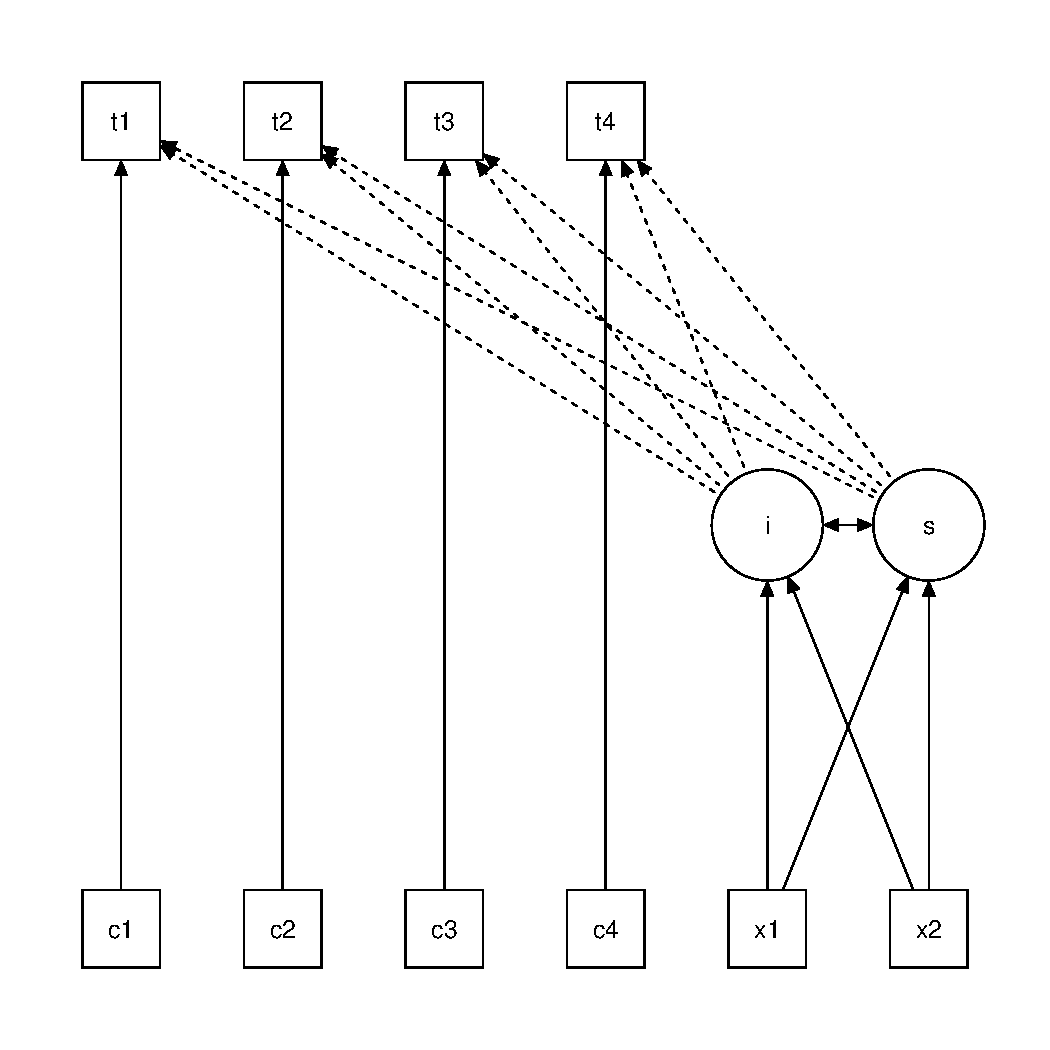
\includegraphics{figure/growth-1.pdf}

The corresponding syntax is the following:

\begin{verbatim}
# intercept and slope
# with fixed coefficients
  i =~ 1*t1 + 1*t2 + 1*t3 + 1*t4
  s =~ 0*t1 + 1*t2 + 2*t3 + 3*t4
# regressions
  i ~ x1 + x2
  s ~ x1 + x2
# time-varying covariates
  t1 ~ c1
  t2 ~ c2
  t3 ~ c3
  t4 ~ c4
\end{verbatim}

For ease of copy/pasting, the complete R code needed to specify and fit
this linear growth model with a time-varying covariate is printed again
below:

\begin{Shaded}
\begin{Highlighting}[]
\CommentTok{# a linear growth model with a time-varying covariate}
\NormalTok{model <-}\StringTok{ '}
\StringTok{  # intercept and slope with fixed coefficients}
\StringTok{    i =~ 1*t1 + 1*t2 + 1*t3 + 1*t4}
\StringTok{    s =~ 0*t1 + 1*t2 + 2*t3 + 3*t4}
\StringTok{  # regressions}
\StringTok{    i ~ x1 + x2}
\StringTok{    s ~ x1 + x2}
\StringTok{  # time-varying covariates}
\StringTok{    t1 ~ c1}
\StringTok{    t2 ~ c2}
\StringTok{    t3 ~ c3}
\StringTok{    t4 ~ c4}
\StringTok{'}
\NormalTok{fit <-}\StringTok{ }\KeywordTok{growth}\NormalTok{(model, }\DataTypeTok{data =}\NormalTok{ Demo.growth)}
\KeywordTok{summary}\NormalTok{(fit)}
\end{Highlighting}
\end{Shaded}


\section{Using categorical variables}
Binary, ordinal and nominal variables are considered categorical (not
continuous). It makes a big difference if these categorical variables
are exogenous (independent) or endogenous (dependent) in the model.

\hypertarget{exogenous-categorical-variables}{%
\paragraph{Exogenous categorical
variables}\label{exogenous-categorical-variables}}

If you have a binary exogenous covariate (say, gender), all you need to
do is to recode it as a dummy (0/1) variable. Just like you would do in
a classic regression model. If you have an exogenous ordinal variable,
you can use a coding scheme reflecting the order (say, 1,2,3,\ldots) and
treat it as any other (numeric) covariate. If you have a nominal
categorical variable with \(K > 2\) levels, you need to replace it by a
set of \(K-1\) dummy variables, again, just like you would do in
classical regression.

\hypertarget{endogenous-categorical-variables}{%
\paragraph{Endogenous categorical
variables}\label{endogenous-categorical-variables}}

The lavaan 0.5 series can deal with binary and ordinal (but not nominal)
endogenous variables. There are two ways to communicate to lavaan that
some of the endogenous variables are to be treated as categorical:

\begin{enumerate}
\def\labelenumi{\arabic{enumi}.}
\item
  declare them as `ordered' (using the \texttt{ordered} function, which
  is part of base R) in your data.frame before you run the analysis; for
  example, if you need to declare four variables (say, \texttt{item1},
  \texttt{item2}, \texttt{item3}, \texttt{item4}) as ordinal in your
  data.frame (called \texttt{Data}), you can use something like:

\begin{Shaded}
\begin{Highlighting}[]
\NormalTok{Data[,}\FunctionTok{c}\NormalTok{(}\StringTok{"item1"}\NormalTok{,}
        \StringTok{"item2"}\NormalTok{,}
        \StringTok{"item3"}\NormalTok{,}
        \StringTok{"item4"}\NormalTok{)] }\OtherTok{\textless{}{-}}
    \FunctionTok{lapply}\NormalTok{(Data[,}\FunctionTok{c}\NormalTok{(}\StringTok{"item1"}\NormalTok{,}
                   \StringTok{"item2"}\NormalTok{,}
                   \StringTok{"item3"}\NormalTok{,}
                   \StringTok{"item4"}\NormalTok{)], ordered)}
\end{Highlighting}
\end{Shaded}
\item
  use the \texttt{ordered} argument when using one of the fitting
  functions (cfa/sem/growth/lavaan), for example, if you have four
  binary or ordinal variables (say, \texttt{item1}, \texttt{item2},
  \texttt{item3}, \texttt{item4}), you can use:

\begin{Shaded}
\begin{Highlighting}[]
\NormalTok{fit }\OtherTok{\textless{}{-}} \FunctionTok{cfa}\NormalTok{(myModel, }\AttributeTok{data =}\NormalTok{ myData,}
           \AttributeTok{ordered =} \FunctionTok{c}\NormalTok{(}\StringTok{"item1"}\NormalTok{,}\StringTok{"item2"}\NormalTok{,}
                       \StringTok{"item3"}\NormalTok{,}\StringTok{"item4"}\NormalTok{))}
\end{Highlighting}
\end{Shaded}
\end{enumerate}

If all the (endogenous) variables are to be treated as categorical, you
can use \texttt{ordered\ =\ TRUE} as a shortcut.

When the \texttt{ordered=} argument is used, lavaan will automatically
switch to the \texttt{WLSMV} estimator: it will use diagonally weighted
least squares (\texttt{DWLS}) to estimate the model parameters, but it
will use the full weight matrix to compute robust standard errors, and a
mean- and variance-adjusted test stastistic. Other options are
unweighted least squares (ULSMV), or pairwise maximum likelihood (PML).
Full information maximum likelihood is currently not supported.

\section{Using a covariance matrix as input}
If you have no full dataset, but you do have a sample covariance matrix,
you can still fit your model. If you wish to add a mean structure, you
need to provide a mean vector too. Importantly, if only sample
statistics are provided, you must specify the number of observations
that were used to compute the sample moments. The following example
illustrates the use of a sample covariance matrix as input. First, we
read in the lower half of the covariance matrix (including the
diagonal):

\begin{Shaded}
\begin{Highlighting}[]
\NormalTok{lower }\OtherTok{\textless{}{-}} \StringTok{\textquotesingle{}}
\StringTok{ 11.834}
\StringTok{  6.947   9.364}
\StringTok{  6.819   5.091  12.532}
\StringTok{  4.783   5.028   7.495   9.986}
\StringTok{ {-}3.839  {-}3.889  {-}3.841  {-}3.625  9.610}
\StringTok{{-}21.899 {-}18.831 {-}21.748 {-}18.775 35.522 450.288 \textquotesingle{}}

\NormalTok{wheaton.cov }\OtherTok{\textless{}{-}} 
    \FunctionTok{getCov}\NormalTok{(lower, }\AttributeTok{names =} \FunctionTok{c}\NormalTok{(}\StringTok{"anomia67"}\NormalTok{, }\StringTok{"powerless67"}\NormalTok{, }
                            \StringTok{"anomia71"}\NormalTok{, }\StringTok{"powerless71"}\NormalTok{,}
                            \StringTok{"education"}\NormalTok{, }\StringTok{"sei"}\NormalTok{))}
\end{Highlighting}
\end{Shaded}

The \texttt{getCov()} function makes it easy to create a full covariance
matrix (including variable names) if you only have the lower-half
elements (perhaps pasted from a textbook or a paper). Note that the
lower-half elements are written between two single quotes. Therefore,
you have some additional flexibility. You can add comments, and blank
lines. If the numbers are separated by a comma, or a semi-colon, that is
fine too. For more information about \texttt{getCov()}, see the online
manual page.

Next, we can specify our model, estimate it, and request a summary of
the results:

\begin{Shaded}
\begin{Highlighting}[]
\CommentTok{\# classic wheaton et al. model}
\NormalTok{wheaton.model }\OtherTok{\textless{}{-}} \StringTok{\textquotesingle{}}
\StringTok{  \# latent variables}
\StringTok{    ses     =\textasciitilde{} education + sei}
\StringTok{    alien67 =\textasciitilde{} anomia67 + powerless67}
\StringTok{    alien71 =\textasciitilde{} anomia71 + powerless71}
\StringTok{  \# regressions}
\StringTok{    alien71 \textasciitilde{} alien67 + ses}
\StringTok{    alien67 \textasciitilde{} ses}
\StringTok{  \# correlated residuals}
\StringTok{    anomia67 \textasciitilde{}\textasciitilde{} anomia71}
\StringTok{    powerless67 \textasciitilde{}\textasciitilde{} powerless71}
\StringTok{\textquotesingle{}}
\NormalTok{fit }\OtherTok{\textless{}{-}} \FunctionTok{sem}\NormalTok{(wheaton.model, }
           \AttributeTok{sample.cov =}\NormalTok{ wheaton.cov, }
           \AttributeTok{sample.nobs =} \DecValTok{932}\NormalTok{)}
\FunctionTok{summary}\NormalTok{(fit, }\AttributeTok{standardized =} \ConstantTok{TRUE}\NormalTok{)}
\end{Highlighting}
\end{Shaded}

\begin{verbatim}
lavaan 0.6-11 ended normally after 84 iterations

  Estimator                                         ML
  Optimization method                           NLMINB
  Number of model parameters                        17
                                                      
  Number of observations                           932
                                                      
Model Test User Model:
                                                      
  Test statistic                                 4.735
  Degrees of freedom                                 4
  P-value (Chi-square)                           0.316

Parameter Estimates:

  Standard errors                             Standard
  Information                                 Expected
  Information saturated (h1) model          Structured

Latent Variables:
                   Estimate  Std.Err  z-value  P(>|z|)   Std.lv  Std.all
  ses =~                                                                
    education         1.000                               2.607    0.842
    sei               5.219    0.422   12.364    0.000   13.609    0.642
  alien67 =~                                                            
    anomia67          1.000                               2.663    0.774
    powerless67       0.979    0.062   15.895    0.000    2.606    0.852
  alien71 =~                                                            
    anomia71          1.000                               2.850    0.805
    powerless71       0.922    0.059   15.498    0.000    2.628    0.832

Regressions:
                   Estimate  Std.Err  z-value  P(>|z|)   Std.lv  Std.all
  alien71 ~                                                             
    alien67           0.607    0.051   11.898    0.000    0.567    0.567
    ses              -0.227    0.052   -4.334    0.000   -0.207   -0.207
  alien67 ~                                                             
    ses              -0.575    0.056  -10.195    0.000   -0.563   -0.563

Covariances:
                   Estimate  Std.Err  z-value  P(>|z|)   Std.lv  Std.all
 .anomia67 ~~                                                           
   .anomia71          1.623    0.314    5.176    0.000    1.623    0.356
 .powerless67 ~~                                                        
   .powerless71       0.339    0.261    1.298    0.194    0.339    0.121

Variances:
                   Estimate  Std.Err  z-value  P(>|z|)   Std.lv  Std.all
   .education         2.801    0.507    5.525    0.000    2.801    0.292
   .sei             264.597   18.126   14.597    0.000  264.597    0.588
   .anomia67          4.731    0.453   10.441    0.000    4.731    0.400
   .powerless67       2.563    0.403    6.359    0.000    2.563    0.274
   .anomia71          4.399    0.515    8.542    0.000    4.399    0.351
   .powerless71       3.070    0.434    7.070    0.000    3.070    0.308
    ses               6.798    0.649   10.475    0.000    1.000    1.000
   .alien67           4.841    0.467   10.359    0.000    0.683    0.683
   .alien71           4.083    0.404   10.104    0.000    0.503    0.503
\end{verbatim}

\hypertarget{the-sample.cov.rescale-argument}{%
\paragraph{\texorpdfstring{The \texttt{sample.cov.rescale}
argument}{The sample.cov.rescale argument}}\label{the-sample.cov.rescale-argument}}

If the estimator is \texttt{ML} (the default), then the sample
variance-covariance matrix will be rescaled by a factor (N-1)/N. The
reasoning is the following: the elements in a sample variance-covariance
matrix have (usually) been divided by N-1. But the (normal-based) ML
estimator would divide the elements by N. Therefore, we need to rescale.
If you don't want this to happen (for example in a simulation study),
you can provide the argument \texttt{sample.cov.rescale\ =\ FALSE}.

\hypertarget{multiple-groups}{%
\paragraph{Multiple groups}\label{multiple-groups}}

If you have multiple groups, the \texttt{sample.cov} argument must be a
list containing the sample variance-covariance matrix of each group as a
separate element in the list. If a mean structure is needed, the
\texttt{sample.mean} argument must be a list containing the sample means
of each group. Finally, the \texttt{sample.nobs} argument can be either
a list or an integer vector containing the number of observations for
each group.

\section{Estimators, standard errors and missing values}
\hypertarget{estimators}{%
\paragraph{Estimators}\label{estimators}}

If all data is continuous, the default estimator in the lavaan package
is maximum likelihood (\texttt{estimator\ =\ "ML"}). Alternative
estimators available in lavaan are:

\begin{itemize}
\tightlist
\item
  \texttt{"GLS"}: generalized least squares. For complete data only.
\item
  \texttt{"WLS"}: weighted least squares (sometimes called ADF
  estimation). For complete data only.
\item
  \texttt{"DWLS"}: diagonally weighted least squares
\item
  \texttt{"ULS"}: unweighted least squares
\item
  \texttt{"DLS"}: distributionally-weighted least squares
\item
  \texttt{"PML"}: pairwise maximum likelihood
\end{itemize}

Many estimators have `robust' variants, meaning that they provide robust
standard errors and a scaled test statistic. For example, for the
maximum likelihood estimator, lavaan provides the following robust
variants:

\begin{itemize}
\tightlist
\item
  \texttt{"MLM"}: maximum likelihood estimation with robust standard
  errors and a Satorra-Bentler scaled test statistic. For complete data
  only.
\item
  \texttt{"MLMVS"}: maximum likelihood estimation with robust standard
  errors and a mean- and variance adjusted test statistic (aka the
  Satterthwaite approach). For complete data only.
\item
  \texttt{"MLMV"}: maximum likelihood estimation with robust standard
  errors and a mean- and variance adjusted test statistic (using a
  scale-shifted approach). For complete data only.
\item
  \texttt{"MLF"}: for maximum likelihood estimation with standard errors
  based on the first-order derivatives, and a conventional test
  statistic. For both complete and incomplete data.
\item
  \texttt{"MLR"}: maximum likelihood estimation with robust
  (Huber-White) standard errors and a scaled test statistic that is
  (asymptotically) equal to the Yuan-Bentler test statistic. For both
  complete and incomplete data.
\end{itemize}

For the \texttt{DWLS} and \texttt{ULS} estimators, lavaan also provides
`robust' variants: \texttt{WLSM}, \texttt{WLSMVS}, \texttt{WLSMV},
\texttt{ULSM}, \texttt{ULSMVS}, \texttt{ULSMV}. Note that for the robust
\texttt{WLS} variants, we use the diagonal of the weight matrix for
estimation, but we use the full weight matrix to correct the standard
errors and to compute the test statistic.

\hypertarget{ml-estimation-wishart-versus-normal}{%
\paragraph{ML estimation: Wishart versus
Normal}\label{ml-estimation-wishart-versus-normal}}

If maximum likelihood estimation is used (\texttt{"ML"} or any of its
robusts variants), the default behavior of lavaan is to base the
analysis on the so-called \emph{biased} sample covariance matrix, where
the elements are divided by N instead of N-1. This is done internally,
and should not be done by the user. In addition, the chi-square
statistic is computed by multiplying the minimum function value with a
factor N (instead of N-1). If you prefer to use an unbiased covariance
matrix, and \(N-1\) as the multiplier to compute the chi-square
statistic, you need to specify the \texttt{likelihood\ =\ "wishart"}
argument when calling the fitting functions. For example:

\begin{Shaded}
\begin{Highlighting}[]
\NormalTok{fit }\OtherTok{\textless{}{-}} \FunctionTok{cfa}\NormalTok{(HS.model, }
           \AttributeTok{data =}\NormalTok{ HolzingerSwineford1939, }
           \AttributeTok{likelihood =} \StringTok{"wishart"}\NormalTok{)}
\NormalTok{fit}
\end{Highlighting}
\end{Shaded}

\begin{verbatim}
lavaan 0.6-11 ended normally after 35 iterations

  Estimator                                         ML
  Optimization method                           NLMINB
  Number of model parameters                        21
                                                      
  Number of observations                           301
                                                      
Model Test User Model:
                                                      
  Test statistic                                85.022
  Degrees of freedom                                24
  P-value (Chi-square)                           0.000
\end{verbatim}

The value of the test statistic will be closer to the value reported by
programs like EQS, LISREL or AMOS, since they all use the `Wishart'
approach when using the maximum likelihood estimator. The program Mplus,
on the other hand, uses the `normal' approach to maximum likelihood
estimation.

\hypertarget{missing-values}{%
\paragraph{Missing values}\label{missing-values}}

If the data contain missing values, the default behavior is listwise
deletion. If the missing mechanism is MCAR (missing completely at
random) or MAR (missing at random), the lavaan package provides
case-wise (or `full information') maximum likelihood estimation. You can
turn this feature on, by using the argument \texttt{missing\ =\ "ML"}
when calling the fitting function. An unrestricted (h1) model will
automatically be estimated, so that all common fit indices are
available.

\hypertarget{standard-errors}{%
\paragraph{Standard errors}\label{standard-errors}}

Standard errors are (by default) based on the expected information
matrix. The only exception is when data are missing and full information
ML is used (via \texttt{missing\ =\ "ML"}). In this case, the observed
information matrix is used to compute the standard errors. The user can
change this behavior by using the \texttt{information} argument.

Robust standard errors can be requested explicitly by using
\texttt{se\ =\ "robust"}. Similarly, robust test statistics can be
requested explicitly by using \texttt{test\ =\ "robust"}. Many more
options are possible. See the help page:

\begin{Shaded}
\begin{Highlighting}[]
\NormalTok{?lavOptions}
\end{Highlighting}
\end{Shaded}

\hypertarget{bootstrapping}{%
\paragraph{Bootstrapping}\label{bootstrapping}}

There are two ways for using the bootstrap in lavaan. Either you can set
\texttt{se\ =\ "bootstrap"} or \texttt{test\ =\ "bootstrap"} when
fitting the model (and you will get bootstrap standard errors, and/or a
bootstrap based p-value respectively), or you can you the
\texttt{bootstrapLavaan()} function, which needs an already fitted
lavaan object. The latter function can be used to `bootstrap' any
statistic (or vector of statistics) that you can extract from a fitted
lavaan object.

\section{Indirect effects and mediation analysis}
Consider a classical mediation setup with three variables: Y is the
dependent variable, X is the predictor, and M is a mediator. For
illustration, we create a toy dataset containing these three variables,
and fit a path analysis model that includes the direct effect of X on Y
and the indirect effect of X on Y via M.

\begin{Shaded}
\begin{Highlighting}[]
\FunctionTok{set.seed}\NormalTok{(}\DecValTok{1234}\NormalTok{)}
\NormalTok{X }\OtherTok{\textless{}{-}} \FunctionTok{rnorm}\NormalTok{(}\DecValTok{100}\NormalTok{)}
\NormalTok{M }\OtherTok{\textless{}{-}} \FloatTok{0.5}\SpecialCharTok{*}\NormalTok{X }\SpecialCharTok{+} \FunctionTok{rnorm}\NormalTok{(}\DecValTok{100}\NormalTok{)}
\NormalTok{Y }\OtherTok{\textless{}{-}} \FloatTok{0.7}\SpecialCharTok{*}\NormalTok{M }\SpecialCharTok{+} \FunctionTok{rnorm}\NormalTok{(}\DecValTok{100}\NormalTok{)}
\NormalTok{Data }\OtherTok{\textless{}{-}} \FunctionTok{data.frame}\NormalTok{(}\AttributeTok{X =}\NormalTok{ X, }\AttributeTok{Y =}\NormalTok{ Y, }\AttributeTok{M =}\NormalTok{ M)}
\NormalTok{model }\OtherTok{\textless{}{-}} \StringTok{\textquotesingle{} \# direct effect}
\StringTok{             Y \textasciitilde{} c*X}
\StringTok{           \# mediator}
\StringTok{             M \textasciitilde{} a*X}
\StringTok{             Y \textasciitilde{} b*M}
\StringTok{           \# indirect effect (a*b)}
\StringTok{             ab := a*b}
\StringTok{           \# total effect}
\StringTok{             total := c + (a*b)}
\StringTok{         \textquotesingle{}}
\NormalTok{fit }\OtherTok{\textless{}{-}} \FunctionTok{sem}\NormalTok{(model, }\AttributeTok{data =}\NormalTok{ Data)}
\FunctionTok{summary}\NormalTok{(fit)}
\end{Highlighting}
\end{Shaded}

\begin{verbatim}
lavaan 0.6-11 ended normally after 1 iterations

  Estimator                                         ML
  Optimization method                           NLMINB
  Number of model parameters                         5
                                                      
  Number of observations                           100
                                                      
Model Test User Model:
                                                      
  Test statistic                                 0.000
  Degrees of freedom                                 0

Parameter Estimates:

  Standard errors                             Standard
  Information                                 Expected
  Information saturated (h1) model          Structured

Regressions:
                   Estimate  Std.Err  z-value  P(>|z|)
  Y ~                                                 
    X          (c)    0.036    0.104    0.348    0.728
  M ~                                                 
    X          (a)    0.474    0.103    4.613    0.000
  Y ~                                                 
    M          (b)    0.788    0.092    8.539    0.000

Variances:
                   Estimate  Std.Err  z-value  P(>|z|)
   .Y                 0.898    0.127    7.071    0.000
   .M                 1.054    0.149    7.071    0.000

Defined Parameters:
                   Estimate  Std.Err  z-value  P(>|z|)
    ab                0.374    0.092    4.059    0.000
    total             0.410    0.125    3.287    0.001
\end{verbatim}

The example illustrates the use of the \texttt{":="} operator in the
lavaan model syntax. This operator `defines' new parameters which take
on values that are an arbitrary function of the original model
parameters. The function, however, must be specified in terms of the
parameter \emph{labels} that are explicitly mentioned in the model
syntax. By default, the standard errors for these defined parameters are
computed by using the so-called Delta method. As with other models,
bootstrap standard errors can be requested simply by specifying
\texttt{se\ =\ "bootstrap"} in the fitting function.

\section{Modification Indices}
Modification indices can be requested by adding the argument
\texttt{modindices\ =\ TRUE} in the \texttt{summary()} call, or by
calling the function \texttt{modindices()} directly. By default,
modification indices are printed out for each nonfree (or fixed-to-zero)
parameter. The modification indices are supplemented by the expected
parameter change (EPC) values (column \texttt{epc}). The last three
columns contain the standardized EPC values (\texttt{sepc.lv}: only
standardizing the latent variables; \texttt{sepc.all}: standardizing all
variables; \texttt{sepc.nox}: standardizing all but exogenous observed
variables).

A typical use of the \texttt{modindices()} function is as follows:

\begin{Shaded}
\begin{Highlighting}[]
\NormalTok{fit }\OtherTok{\textless{}{-}} \FunctionTok{cfa}\NormalTok{(HS.model,}
           \AttributeTok{data =}\NormalTok{ HolzingerSwineford1939)}
\FunctionTok{modindices}\NormalTok{(fit, }\AttributeTok{sort =} \ConstantTok{TRUE}\NormalTok{, }\AttributeTok{maximum.number =} \DecValTok{5}\NormalTok{)}
\end{Highlighting}
\end{Shaded}

\begin{verbatim}
       lhs op rhs     mi    epc sepc.lv sepc.all sepc.nox
30  visual =~  x9 36.411  0.577   0.519    0.515    0.515
76      x7 ~~  x8 34.145  0.536   0.536    0.859    0.859
28  visual =~  x7 18.631 -0.422  -0.380   -0.349   -0.349
78      x8 ~~  x9 14.946 -0.423  -0.423   -0.805   -0.805
33 textual =~  x3  9.151 -0.272  -0.269   -0.238   -0.238
\end{verbatim}

This will print out the top 5 parameters (that can be added to the
model) that result in the largest modification index, sorted from high
to low.

The \texttt{modindices()} function returns a data frame, which you can
sort or filter to extract what you want. For example, to see only the
modification indices for the factor loadings, you can use something like
this:

\begin{Shaded}
\begin{Highlighting}[]
\NormalTok{fit }\OtherTok{\textless{}{-}} \FunctionTok{cfa}\NormalTok{(HS.model, }
           \AttributeTok{data =}\NormalTok{ HolzingerSwineford1939)}
\NormalTok{mi }\OtherTok{\textless{}{-}} \FunctionTok{modindices}\NormalTok{(fit)}
\NormalTok{mi[mi}\SpecialCharTok{$}\NormalTok{op }\SpecialCharTok{==} \StringTok{"=\textasciitilde{}"}\NormalTok{,]}
\end{Highlighting}
\end{Shaded}

\begin{verbatim}
       lhs op rhs     mi    epc sepc.lv sepc.all sepc.nox
25  visual =~  x4  1.211  0.077   0.069    0.059    0.059
26  visual =~  x5  7.441 -0.210  -0.189   -0.147   -0.147
27  visual =~  x6  2.843  0.111   0.100    0.092    0.092
28  visual =~  x7 18.631 -0.422  -0.380   -0.349   -0.349
29  visual =~  x8  4.295 -0.210  -0.189   -0.187   -0.187
30  visual =~  x9 36.411  0.577   0.519    0.515    0.515
31 textual =~  x1  8.903  0.350   0.347    0.297    0.297
32 textual =~  x2  0.017 -0.011  -0.011   -0.010   -0.010
33 textual =~  x3  9.151 -0.272  -0.269   -0.238   -0.238
34 textual =~  x7  0.098 -0.021  -0.021   -0.019   -0.019
35 textual =~  x8  3.359 -0.121  -0.120   -0.118   -0.118
36 textual =~  x9  4.796  0.138   0.137    0.136    0.136
37   speed =~  x1  0.014  0.024   0.015    0.013    0.013
38   speed =~  x2  1.580 -0.198  -0.123   -0.105   -0.105
39   speed =~  x3  0.716  0.136   0.084    0.075    0.075
40   speed =~  x4  0.003 -0.005  -0.003   -0.003   -0.003
41   speed =~  x5  0.201 -0.044  -0.027   -0.021   -0.021
42   speed =~  x6  0.273  0.044   0.027    0.025    0.025
\end{verbatim}

It is important to realize that the \texttt{modindices()} function will
only consider fixed-to-zero parameters. If you have equality constraints
in the model, and you wish to examine what happens if you release all
(or some) of these equality constraints, use the \texttt{lavTestScore()}
function.

\section{Extracting information from a fitted model}
The \texttt{summary()} function gives a nice overview of a fitted model,
but is for display only. If you need the actual numbers for further
processing, you may prefer to use one of several `extractor' functions.
We have already seen the \texttt{coef()} function which extracts the
estimated parameters of a fitted model. Other extractor functions are
discussed below.

\hypertarget{parameterestimates}{%
\paragraph{parameterEstimates}\label{parameterestimates}}

The \texttt{parameterEstimates} function extracts not only the values of
the estimated parameters, but also the standard errors, the z-values,
the standardized parameter values, and returns everything conveniently
as a data frame. For example:

\begin{Shaded}
\begin{Highlighting}[]
\NormalTok{fit <-}\StringTok{ }\KeywordTok{cfa}\NormalTok{(HS.model, }\DataTypeTok{data=}\NormalTok{HolzingerSwineford1939)}
\KeywordTok{parameterEstimates}\NormalTok{(fit)}
\end{Highlighting}
\end{Shaded}

\begin{verbatim}
       lhs op     rhs   est    se      z pvalue ci.lower ci.upper
1   visual =~      x1 1.000 0.000     NA     NA    1.000    1.000
2   visual =~      x2 0.554 0.100  5.554      0    0.358    0.749
3   visual =~      x3 0.729 0.109  6.685      0    0.516    0.943
4  textual =~      x4 1.000 0.000     NA     NA    1.000    1.000
5  textual =~      x5 1.113 0.065 17.014      0    0.985    1.241
6  textual =~      x6 0.926 0.055 16.703      0    0.817    1.035
7    speed =~      x7 1.000 0.000     NA     NA    1.000    1.000
8    speed =~      x8 1.180 0.165  7.152      0    0.857    1.503
9    speed =~      x9 1.082 0.151  7.155      0    0.785    1.378
10      x1 ~~      x1 0.549 0.114  4.833      0    0.326    0.772
11      x2 ~~      x2 1.134 0.102 11.146      0    0.934    1.333
12      x3 ~~      x3 0.844 0.091  9.317      0    0.667    1.022
13      x4 ~~      x4 0.371 0.048  7.779      0    0.278    0.465
14      x5 ~~      x5 0.446 0.058  7.642      0    0.332    0.561
15      x6 ~~      x6 0.356 0.043  8.277      0    0.272    0.441
16      x7 ~~      x7 0.799 0.081  9.823      0    0.640    0.959
17      x8 ~~      x8 0.488 0.074  6.573      0    0.342    0.633
18      x9 ~~      x9 0.566 0.071  8.003      0    0.427    0.705
19  visual ~~  visual 0.809 0.145  5.564      0    0.524    1.094
20 textual ~~ textual 0.979 0.112  8.737      0    0.760    1.199
21   speed ~~   speed 0.384 0.086  4.451      0    0.215    0.553
22  visual ~~ textual 0.408 0.074  5.552      0    0.264    0.552
23  visual ~~   speed 0.262 0.056  4.660      0    0.152    0.373
24 textual ~~   speed 0.173 0.049  3.518      0    0.077    0.270
\end{verbatim}

\hypertarget{standardizedsolution}{%
\paragraph{standardizedSolution}\label{standardizedsolution}}

The \texttt{standardizedSolution()} function is similar to the
\texttt{parameterEstimates()} function, but only shows the
unstandardized and standardized parameter estimates.

\hypertarget{fitted.values}{%
\paragraph{fitted.values}\label{fitted.values}}

The \texttt{fitted()} and \texttt{fitted.values()} functions return the
model-implied (fitted) covariance matrix (and mean vector) of a fitted
model:

\begin{Shaded}
\begin{Highlighting}[]
\NormalTok{fit <-}\StringTok{ }\KeywordTok{cfa}\NormalTok{(HS.model, }\DataTypeTok{data=}\NormalTok{HolzingerSwineford1939)}
\KeywordTok{fitted}\NormalTok{(fit)}
\end{Highlighting}
\end{Shaded}

\begin{verbatim}
$cov
   x1    x2    x3    x4    x5    x6    x7    x8    x9   
x1 1.358                                                
x2 0.448 1.382                                          
x3 0.590 0.327 1.275                                    
x4 0.408 0.226 0.298 1.351                              
x5 0.454 0.252 0.331 1.090 1.660                        
x6 0.378 0.209 0.276 0.907 1.010 1.196                  
x7 0.262 0.145 0.191 0.173 0.193 0.161 1.183            
x8 0.309 0.171 0.226 0.205 0.228 0.190 0.453 1.022      
x9 0.284 0.157 0.207 0.188 0.209 0.174 0.415 0.490 1.015

$mean
x1 x2 x3 x4 x5 x6 x7 x8 x9 
 0  0  0  0  0  0  0  0  0 
\end{verbatim}

\hypertarget{residuals}{%
\paragraph{residuals}\label{residuals}}

The \texttt{resid()} or \texttt{residuals()} functions return
(unstandardized) residuals of a fitted model. This is simply the
difference between the observed and implied covariance matrix and mean
vector. If the estimator is maximum likelihood, it is also possible to
obtain the normalized and the standardized residuals (note: you may
observe several \texttt{NA} values, but they can be safely ignored)

\begin{Shaded}
\begin{Highlighting}[]
\NormalTok{fit <-}\StringTok{ }\KeywordTok{cfa}\NormalTok{(HS.model, }\DataTypeTok{data=}\NormalTok{HolzingerSwineford1939)}
\KeywordTok{resid}\NormalTok{(fit, }\DataTypeTok{type=}\StringTok{"standardized"}\NormalTok{)}
\end{Highlighting}
\end{Shaded}

\begin{verbatim}
$type
[1] "standardized"

$cov
   x1     x2     x3     x4     x5     x6     x7     x8     x9    
x1     NA                                                        
x2 -2.196  0.000                                                 
x3 -1.199  2.692  0.000                                          
x4  2.465 -0.283 -1.948  0.000                                   
x5 -0.362 -0.610 -4.443  0.856  0.000                            
x6  2.032  0.661 -0.701     NA  0.633  0.000                     
x7 -3.787 -3.800 -1.882  0.839 -0.837 -0.321  0.000              
x8 -1.456 -1.137 -0.305 -2.049 -1.100 -0.635  3.804  0.000       
x9  4.062  1.517  3.328  1.237  1.723  1.436 -2.771     NA  0.000

$mean
x1 x2 x3 x4 x5 x6 x7 x8 x9 
 0  0  0  0  0  0  0  0  0 
\end{verbatim}

\hypertarget{vcov}{%
\paragraph{vcov}\label{vcov}}

The function \texttt{vcov()} returns the estimated covariance matrix of
the parameter estimates.

\hypertarget{aic-and-bic}{%
\paragraph{AIC and BIC}\label{aic-and-bic}}

The \texttt{AIC()} and \texttt{BIC()} functions return the AIC and BIC
values of a fitted model.

\hypertarget{fitmeasures}{%
\paragraph{fitMeasures}\label{fitmeasures}}

The \texttt{fitMeasures()} function returns all the fit measures
computed by lavaan as a named numeric vector.

\begin{Shaded}
\begin{Highlighting}[]
\NormalTok{fit <-}\StringTok{ }\KeywordTok{cfa}\NormalTok{(HS.model, }\DataTypeTok{data=}\NormalTok{HolzingerSwineford1939)}
\KeywordTok{fitMeasures}\NormalTok{(fit)}
\end{Highlighting}
\end{Shaded}

\begin{verbatim}
               npar                fmin               chisq 
             21.000               0.142              85.306 
                 df              pvalue      baseline.chisq 
             24.000               0.000             918.852 
        baseline.df     baseline.pvalue                 cfi 
             36.000               0.000               0.931 
                tli                nnfi                 rfi 
              0.896               0.896               0.861 
                nfi                pnfi                 ifi 
              0.907               0.605               0.931 
                rni                logl   unrestricted.logl 
              0.931           -3737.745           -3695.092 
                aic                 bic              ntotal 
           7517.490            7595.339             301.000 
               bic2               rmsea      rmsea.ci.lower 
           7528.739               0.092               0.071 
     rmsea.ci.upper        rmsea.pvalue                 rmr 
              0.114               0.001               0.082 
         rmr_nomean                srmr        srmr_bentler 
              0.082               0.065               0.065 
srmr_bentler_nomean         srmr_bollen  srmr_bollen_nomean 
              0.065               0.065               0.065 
         srmr_mplus   srmr_mplus_nomean               cn_05 
              0.065               0.065             129.490 
              cn_01                 gfi                agfi 
            152.654               0.943               0.894 
               pgfi                 mfi                ecvi 
              0.503               0.903               0.423 
\end{verbatim}

If you only want the value of a single fit measure, say, the CFI, you
give the name (in lower case) as the second argument:

\begin{Shaded}
\begin{Highlighting}[]
\NormalTok{fit <-}\StringTok{ }\KeywordTok{cfa}\NormalTok{(HS.model, }\DataTypeTok{data=}\NormalTok{HolzingerSwineford1939)}
\KeywordTok{fitMeasures}\NormalTok{(fit, }\StringTok{"cfi"}\NormalTok{)}
\end{Highlighting}
\end{Shaded}

\begin{verbatim}
  cfi 
0.931 
\end{verbatim}

Or you can provide a vector of fit measures, as in

\begin{Shaded}
\begin{Highlighting}[]
\KeywordTok{fitMeasures}\NormalTok{(fit, }\KeywordTok{c}\NormalTok{(}\StringTok{"cfi"}\NormalTok{,}\StringTok{"rmsea"}\NormalTok{,}\StringTok{"srmr"}\NormalTok{))}
\end{Highlighting}
\end{Shaded}

\begin{verbatim}
  cfi rmsea  srmr 
0.931 0.092 0.065 
\end{verbatim}

\hypertarget{inspect}{%
\paragraph{inspect}\label{inspect}}

If you want to peek inside a fitted lavaan object (the object that is
returned by a call to \texttt{cfa()}, \texttt{sem()}or
\texttt{growth()}), you can use the \texttt{inspect()} function, with a
variety of options. By default, calling \texttt{inspect()} on a fitted
lavaan object returns a list of the model matrices that are used
internally to represent the model. The free parameters are nonzero
integers.

\begin{Shaded}
\begin{Highlighting}[]
\NormalTok{fit <-}\StringTok{ }\KeywordTok{cfa}\NormalTok{(HS.model, }\DataTypeTok{data=}\NormalTok{HolzingerSwineford1939)}
\KeywordTok{inspect}\NormalTok{(fit)}
\end{Highlighting}
\end{Shaded}

\begin{verbatim}
$lambda
   visual textul speed
x1      0      0     0
x2      1      0     0
x3      2      0     0
x4      0      0     0
x5      0      3     0
x6      0      4     0
x7      0      0     0
x8      0      0     5
x9      0      0     6

$theta
   x1 x2 x3 x4 x5 x6 x7 x8 x9
x1  7                        
x2  0  8                     
x3  0  0  9                  
x4  0  0  0 10               
x5  0  0  0  0 11            
x6  0  0  0  0  0 12         
x7  0  0  0  0  0  0 13      
x8  0  0  0  0  0  0  0 14   
x9  0  0  0  0  0  0  0  0 15

$psi
        visual textul speed
visual  16                 
textual 19     17          
speed   20     21     18   
\end{verbatim}

To see the starting values of parameters in each model matrix, type

\begin{Shaded}
\begin{Highlighting}[]
\KeywordTok{inspect}\NormalTok{(fit, }\DataTypeTok{what=}\StringTok{"start"}\NormalTok{)}
\end{Highlighting}
\end{Shaded}

\begin{verbatim}
$lambda
   visual textul speed
x1  1.000  0.000 0.000
x2  0.778  0.000 0.000
x3  1.107  0.000 0.000
x4  0.000  1.000 0.000
x5  0.000  1.133 0.000
x6  0.000  0.924 0.000
x7  0.000  0.000 1.000
x8  0.000  0.000 1.225
x9  0.000  0.000 0.854

$theta
   x1    x2    x3    x4    x5    x6    x7    x8    x9   
x1 0.679                                                
x2 0.000 0.691                                          
x3 0.000 0.000 0.637                                    
x4 0.000 0.000 0.000 0.675                              
x5 0.000 0.000 0.000 0.000 0.830                        
x6 0.000 0.000 0.000 0.000 0.000 0.598                  
x7 0.000 0.000 0.000 0.000 0.000 0.000 0.592            
x8 0.000 0.000 0.000 0.000 0.000 0.000 0.000 0.511      
x9 0.000 0.000 0.000 0.000 0.000 0.000 0.000 0.000 0.508

$psi
        visual textul speed
visual  0.05               
textual 0.00   0.05        
speed   0.00   0.00   0.05 
\end{verbatim}

To see how lavaan internally represents a model, you can type

\begin{Shaded}
\begin{Highlighting}[]
\KeywordTok{inspect}\NormalTok{(fit, }\DataTypeTok{what=}\StringTok{"list"}\NormalTok{)}
\end{Highlighting}
\end{Shaded}

\begin{verbatim}
   id     lhs op     rhs user block group free ustart exo label plabel
1   1  visual =~      x1    1     1     1    0      1   0         .p1.
2   2  visual =~      x2    1     1     1    1     NA   0         .p2.
3   3  visual =~      x3    1     1     1    2     NA   0         .p3.
4   4 textual =~      x4    1     1     1    0      1   0         .p4.
5   5 textual =~      x5    1     1     1    3     NA   0         .p5.
6   6 textual =~      x6    1     1     1    4     NA   0         .p6.
7   7   speed =~      x7    1     1     1    0      1   0         .p7.
8   8   speed =~      x8    1     1     1    5     NA   0         .p8.
9   9   speed =~      x9    1     1     1    6     NA   0         .p9.
10 10      x1 ~~      x1    0     1     1    7     NA   0        .p10.
11 11      x2 ~~      x2    0     1     1    8     NA   0        .p11.
12 12      x3 ~~      x3    0     1     1    9     NA   0        .p12.
13 13      x4 ~~      x4    0     1     1   10     NA   0        .p13.
14 14      x5 ~~      x5    0     1     1   11     NA   0        .p14.
15 15      x6 ~~      x6    0     1     1   12     NA   0        .p15.
16 16      x7 ~~      x7    0     1     1   13     NA   0        .p16.
17 17      x8 ~~      x8    0     1     1   14     NA   0        .p17.
18 18      x9 ~~      x9    0     1     1   15     NA   0        .p18.
19 19  visual ~~  visual    0     1     1   16     NA   0        .p19.
20 20 textual ~~ textual    0     1     1   17     NA   0        .p20.
21 21   speed ~~   speed    0     1     1   18     NA   0        .p21.
22 22  visual ~~ textual    0     1     1   19     NA   0        .p22.
23 23  visual ~~   speed    0     1     1   20     NA   0        .p23.
24 24 textual ~~   speed    0     1     1   21     NA   0        .p24.
   start   est    se
1  1.000 1.000 0.000
2  0.778 0.554 0.100
3  1.107 0.729 0.109
4  1.000 1.000 0.000
5  1.133 1.113 0.065
6  0.924 0.926 0.055
7  1.000 1.000 0.000
8  1.225 1.180 0.165
9  0.854 1.082 0.151
10 0.679 0.549 0.114
11 0.691 1.134 0.102
12 0.637 0.844 0.091
13 0.675 0.371 0.048
14 0.830 0.446 0.058
15 0.598 0.356 0.043
16 0.592 0.799 0.081
17 0.511 0.488 0.074
18 0.508 0.566 0.071
19 0.050 0.809 0.145
20 0.050 0.979 0.112
21 0.050 0.384 0.086
22 0.000 0.408 0.074
23 0.000 0.262 0.056
24 0.000 0.173 0.049
\end{verbatim}

This is equivalent to the \texttt{parTable(fit)} function. The table
that is returned here is called the `parameter table'.

For more inspect options, see the help page for the lavaan class which
you can find by typing the following:

\begin{Shaded}
\begin{Highlighting}[]
\NormalTok{class?lavaan}
\end{Highlighting}
\end{Shaded}


\section{Multilevel SEM}
If the data is clustered, one way to handle the clustering is to use a
multilevel modeling approach. In the SEM framework, this leads to
multilevel SEM. The multilevel capabilities of lavaan are still limited,
but you can fit a two-level SEM with random intercepts (note: only when
all data is continuous and complete; listwise deletion is currently used
for cases with missing values).

\hypertarget{multilevel-sem-model-syntax}{%
\paragraph{Multilevel SEM model
syntax}\label{multilevel-sem-model-syntax}}

To fit a two-level SEM, you must specify a model for both levels, as
follows:

\begin{Shaded}
\begin{Highlighting}[]
\NormalTok{    model <-}\StringTok{ '}
\StringTok{        level: 1}
\StringTok{            fw =~ y1 + y2 + y3}
\StringTok{            fw ~ x1 + x2 + x3}
\StringTok{        level: 2}
\StringTok{            fb =~ y1 + y2 + y3}
\StringTok{            fb ~ w1 + w2}
\StringTok{    '}
\end{Highlighting}
\end{Shaded}

This model syntax contains two blocks, one for level 1, and one for
level 2. Within each block, you can specify a model just like in the
single-level case. To fit this model, using a toy dataset
\texttt{Demo.twolevel} that is part of the lavaan package, you need to
add the \texttt{cluster=} argument to the sem/lavaan function call:

\begin{Shaded}
\begin{Highlighting}[]
\NormalTok{    fit <-}\StringTok{ }\KeywordTok{sem}\NormalTok{(}\DataTypeTok{model =}\NormalTok{ model, }\DataTypeTok{data =}\NormalTok{ Demo.twolevel, }\DataTypeTok{cluster =} \StringTok{"cluster"}\NormalTok{)}
\end{Highlighting}
\end{Shaded}

The output looks similar to a multigroup SEM output, but where the two
groups are now the within and the between level respectively.

\begin{Shaded}
\begin{Highlighting}[]
    \KeywordTok{summary}\NormalTok{(fit)}
\end{Highlighting}
\end{Shaded}

\begin{verbatim}
## lavaan (0.6-1) converged normally after  36 iterations
## 
##   Number of observations                          2500
##   Number of clusters [cluster]                     200
## 
##   Estimator                                         ML
##   Model Fit Test Statistic                       8.092
##   Degrees of freedom                                10
##   P-value (Chi-square)                           0.620
## 
## Parameter Estimates:
## 
##   Information                                 Observed
##   Observed information based on                Hessian
##   Standard Errors                             Standard
## 
## 
## Level 1 [within]:
## 
## Latent Variables:
##                    Estimate  Std.Err  z-value  P(>|z|)
##   fw =~                                               
##     y1                1.000                           
##     y2                0.774    0.034   22.671    0.000
##     y3                0.734    0.033   22.355    0.000
## 
## Regressions:
##                    Estimate  Std.Err  z-value  P(>|z|)
##   fw ~                                                
##     x1                0.510    0.023   22.037    0.000
##     x2                0.407    0.022   18.273    0.000
##     x3                0.205    0.021    9.740    0.000
## 
## Intercepts:
##                    Estimate  Std.Err  z-value  P(>|z|)
##    .y1                0.000                           
##    .y2                0.000                           
##    .y3                0.000                           
##    .fw                0.000                           
## 
## Variances:
##                    Estimate  Std.Err  z-value  P(>|z|)
##    .y1                0.986    0.046   21.591    0.000
##    .y2                1.066    0.039   27.271    0.000
##    .y3                1.011    0.037   27.662    0.000
##    .fw                0.546    0.040   13.539    0.000
## 
## 
## Level 2 [cluster]:
## 
## Latent Variables:
##                    Estimate  Std.Err  z-value  P(>|z|)
##   fb =~                                               
##     y1                1.000                           
##     y2                0.717    0.052   13.824    0.000
##     y3                0.587    0.048   12.329    0.000
## 
## Regressions:
##                    Estimate  Std.Err  z-value  P(>|z|)
##   fb ~                                                
##     w1                0.165    0.079    2.093    0.036
##     w2                0.131    0.076    1.715    0.086
## 
## Intercepts:
##                    Estimate  Std.Err  z-value  P(>|z|)
##    .y1                0.024    0.075    0.327    0.743
##    .y2               -0.016    0.060   -0.269    0.788
##    .y3               -0.042    0.054   -0.777    0.437
##    .fb                0.000                           
## 
## Variances:
##                    Estimate  Std.Err  z-value  P(>|z|)
##    .y1                0.058    0.047    1.213    0.225
##    .y2                0.120    0.031    3.825    0.000
##    .y3                0.149    0.028    5.319    0.000
##    .fb                0.899    0.118    7.592    0.000
\end{verbatim}

After fitting the model, you can inspect the intra-class correlations:

\begin{Shaded}
\begin{Highlighting}[]
    \KeywordTok{lavInspect}\NormalTok{(fit, }\StringTok{"icc"}\NormalTok{)}
\end{Highlighting}
\end{Shaded}

\begin{verbatim}
##    y1    y2    y3    x1    x2    x3 
## 0.331 0.263 0.232 0.000 0.000 0.000
\end{verbatim}

The see the unrestricted (h1) within and between means and covariances,
you can use

\begin{Shaded}
\begin{Highlighting}[]
    \KeywordTok{lavInspect}\NormalTok{(fit, }\StringTok{"h1"}\NormalTok{)}
\end{Highlighting}
\end{Shaded}

\begin{verbatim}
## $within
## $within$cov
##    y1     y2     y3     x1     x2     x3    
## y1  2.000                                   
## y2  0.789  1.674                            
## y3  0.749  0.564  1.557                     
## x1  0.489  0.393  0.376  0.982              
## x2  0.416  0.322  0.299  0.001  1.011       
## x3  0.221  0.160  0.155 -0.006  0.008  1.045
## 
## $within$mean
##     y1     y2     y3     x1     x2     x3 
##  0.001 -0.002 -0.001 -0.007 -0.003  0.020 
## 
## 
## $cluster
## $cluster$cov
##    y1     y2     y3     w1     w2    
## y1  0.992                            
## y2  0.668  0.598                     
## y3  0.548  0.391  0.469              
## w1  0.125  0.119  0.036  0.870       
## w2  0.086  0.057  0.130 -0.128  0.931
## 
## $cluster$mean
##     y1     y2     y3     w1     w2 
##  0.019 -0.017 -0.043  0.052 -0.091
\end{verbatim}

\hypertarget{important-notes}{%
\paragraph{Important notes}\label{important-notes}}

\begin{itemize}
\item
  note that in \texttt{level:\ 1} the colon follows the \texttt{level}
  keyword; if you type \texttt{level\ 1:}, you will get an error
\item
  you must specify a model for each level; the following syntax is not
  allowed and will produce an error:

\begin{Shaded}
\begin{Highlighting}[]
\NormalTok{    model <-}\StringTok{ '}
\StringTok{        level: 1}
\StringTok{            fw =~ y1 + y2 + y3}
\StringTok{            fw ~ x1 + x2 + x3}
\StringTok{        level: 2}
\StringTok{    '}
\end{Highlighting}
\end{Shaded}
\item
  if you do not have a model in mind for level 2, you can specify a
  saturated level by adding all variances and covariances of the
  endogenous variables (here: y1, y2 and y3):

\begin{Shaded}
\begin{Highlighting}[]
\NormalTok{    model <-}\StringTok{ '}
\StringTok{        level: 1}
\StringTok{            fw =~ y1 + y2 + y3}
\StringTok{            fw ~ x1 + x2 + x3}
\StringTok{        level: 2}
\StringTok{            y1 ~~ y1 + y2 + y3}
\StringTok{            y2 ~~ y2 + y3}
\StringTok{            y3 ~~ y3}
\StringTok{    '}
\end{Highlighting}
\end{Shaded}
\end{itemize}

\hypertarget{convergence-issues-and-solutions}{%
\paragraph{Convergence issues and
solutions}\label{convergence-issues-and-solutions}}

By default, the current version of lavaan (0.6) uses a quasi-Newton
procedure to maximize the loglikelihood of the data given the model
(just like in the single-level case). For most model and data
combinations, this will work fine (and fast). However, every now and
then, you may experience convergence issues.

Non-convergence is typically a sign that something is not quite right
with either your model, or your data. Typical settings are: a small
number of clusters, in combination with (almost) no variance of an
endogenous variable at the between level.

However, if you believe nothing is wrong, you may want to try another
optimization procedure. The current version of lavaan allows for using
the Expectation Maximization (EM) algorithm as an alternative. To switch
to the EM algorithm, you can use:

\begin{Shaded}
\begin{Highlighting}[]
\NormalTok{    fit <-}\StringTok{ }\KeywordTok{sem}\NormalTok{(}\DataTypeTok{model =}\NormalTok{ model, }\DataTypeTok{data =}\NormalTok{ Demo.twolevel, }\DataTypeTok{cluster =} \StringTok{"cluster"}\NormalTok{,}
               \DataTypeTok{verbose =} \OtherTok{TRUE}\NormalTok{, }\DataTypeTok{optim.method =} \StringTok{"em"}\NormalTok{)}
\end{Highlighting}
\end{Shaded}

As the EM algorithm is not accelerated yet, this may take a long time.
It is not unusual that more than 10000 iterations are needed to reach a
solution. To control when the EM algorithm stops, you can set the
stopping criteria as follows:

\begin{Shaded}
\begin{Highlighting}[]
\NormalTok{    fit <-}\StringTok{ }\KeywordTok{sem}\NormalTok{(}\DataTypeTok{model =}\NormalTok{ model, }\DataTypeTok{data =}\NormalTok{ Demo.twolevel, }\DataTypeTok{cluster =} \StringTok{"cluster"}\NormalTok{,}
               \DataTypeTok{verbose =} \OtherTok{TRUE}\NormalTok{, }\DataTypeTok{optim.method =} \StringTok{"em"}\NormalTok{, }\DataTypeTok{em.iter.max =} \DecValTok{20000}\NormalTok{,}
               \DataTypeTok{em.fx.tol =} \FloatTok{1e-08}\NormalTok{, }\DataTypeTok{em.dx.tol =} \FloatTok{1e-04}\NormalTok{)}
\end{Highlighting}
\end{Shaded}

The \texttt{em.fx.tol} argument is used to monitor the change in
loglikelihood between the current step and the previous step. If this
change is smaller than \texttt{em.fx.tol}, the algorithm stops. The
\texttt{em.dx.tol} argument is used to monitor the (unscaled) gradient.
When a solution is reached, all elements of the gradient should be near
zero. When the largest gradient element is smaller than
\texttt{em.dx.tol}, the algorithm stops.

A word of caution: the EM algorithm can always be forced to `converge'
(perhaps after changing the stopping criteria), but that does not mean
you have a model/dataset combination that deserves to converge.

\section{ESEM and exploratory factor analysis (EFA)}
If a measurement model contains multiple latent variables (factors), we
usually know which indicators belong to each factor. We call this the
factor structure. Confirmatory factor analysis can be used to check if
this a priori factor structure holds in the data. There are settings,
however, where the factor structure is unclear, and we wish to rotate
the solution in order to find a suitable structure in a given model.
When the model also includes a structural part (i.e., regressions among
the latent variables), this is referred to as exploratory structural
equation modeling or ESEM. If there is only a measurement part, this is
called exploratory factor analysis (EFA). What they have in common is
that the factor structure (for one or more blocks) is found by means of
rotation.

\hypertarget{esem}{%
\paragraph{ESEM}\label{esem}}

To illustrate how ESEM works in lavaan, consider the following syntax:

\begin{Shaded}
\begin{Highlighting}[]
\NormalTok{model }\OtherTok{\textless{}{-}} \StringTok{\textquotesingle{}}
\StringTok{    \# efa block 1}
\StringTok{    efa("efa1")*f1 + }
\StringTok{    efa("efa1")*f2 =\textasciitilde{} x1 + x2 + x3 + x4 + x5 + x6}

\StringTok{    \# efa block 2}
\StringTok{    efa("efa2")*f3 + }
\StringTok{    efa("efa2")*f4 =\textasciitilde{} y1 + y2 + y3 + y4 + y5 + y6}

\StringTok{    \# cfa block}
\StringTok{    f5 =\textasciitilde{} z7 + z8 + z9}
\StringTok{    f6 =\textasciitilde{} z10 + z11 + z12}

\StringTok{    \# regressions}
\StringTok{    f3 \textasciitilde{} f1 + f2}
\StringTok{    f4 \textasciitilde{} f3}
\StringTok{\textquotesingle{}}
\end{Highlighting}
\end{Shaded}

This model syntax defines six latent variables (or factors). For f5 and
f6, the factor structure is known, and they belong to a regular CFA
block. But for f1 and f2, the factor structure is not known, and we will
use a rotation method to find an appropiate structure. The f1 and f2
factors belong together in an EFA block that is (arbitrarily) named
\texttt{efa1}. The \texttt{efa("efa1")*} modifier just before f1 and f2
is used to alert lavaan that these two factors belong to the same EFA
block. The factors f3 and f4 belong to a different EFA block (named
\texttt{efa2}) and will be rotated independently. The structural part of
the model is given as usual. To fit this model, we could call the
\texttt{sem()} function as follows:

\begin{Shaded}
\begin{Highlighting}[]
\NormalTok{fit }\OtherTok{\textless{}{-}} \FunctionTok{sem}\NormalTok{(}\AttributeTok{model =}\NormalTok{ model, }\AttributeTok{data =}\NormalTok{ myData, }\AttributeTok{rotation =} \StringTok{"geomin"}\NormalTok{)}
\end{Highlighting}
\end{Shaded}

Different rotation criteria are available, and many rotation options can
be provided (see the manual page for the \texttt{efa()} function for an
overview).

To illustrate ESEM, we will borrow an example from the Mplus User's
Guide (example 5.25). First we read in the data:

\begin{Shaded}
\begin{Highlighting}[]
\NormalTok{ex5\_25 }\OtherTok{\textless{}{-}} \FunctionTok{read.table}\NormalTok{(}\StringTok{"http://statmodel.com/usersguide/chap5/ex5.25.dat"}\NormalTok{)}
\FunctionTok{names}\NormalTok{(ex5\_25) }\OtherTok{=} \FunctionTok{paste0}\NormalTok{(}\StringTok{"y"}\NormalTok{,}\DecValTok{1}\SpecialCharTok{:}\DecValTok{12}\NormalTok{)}
\end{Highlighting}
\end{Shaded}

The model syntax contains a single EFA block (\texttt{efa1} for factors
f1 and f2) and single CFA block (for f3 and f4):

\begin{Shaded}
\begin{Highlighting}[]
\NormalTok{model }\OtherTok{\textless{}{-}} \StringTok{\textquotesingle{}}
\StringTok{    \# efa block }
\StringTok{    efa("efa1")*f1 + }
\StringTok{    efa("efa1")*f2 =\textasciitilde{} y1 + y2 + y3 + y4 + y5 + y6}

\StringTok{    \# cfa block}
\StringTok{    f3 =\textasciitilde{} y7 + y8 + y9}
\StringTok{    f4 =\textasciitilde{} y10 + y11 + y12}

\StringTok{    \# regressions}
\StringTok{    f3 \textasciitilde{} f1 + f2}
\StringTok{    f4 \textasciitilde{} f3}
\StringTok{\textquotesingle{}}
\end{Highlighting}
\end{Shaded}

The following command illustrates the use of various rotation arguments:

\begin{Shaded}
\begin{Highlighting}[]
\NormalTok{fit }\OtherTok{\textless{}{-}} \FunctionTok{sem}\NormalTok{(}\AttributeTok{model =}\NormalTok{ model, }\AttributeTok{data =}\NormalTok{ ex5\_25, }\AttributeTok{rotation =} \StringTok{"geomin"}\NormalTok{,}
           \CommentTok{\# mimic Mplus}
           \AttributeTok{information =} \StringTok{"observed"}\NormalTok{,}
           \AttributeTok{rotation.args =} \FunctionTok{list}\NormalTok{(}\AttributeTok{rstarts =} \DecValTok{30}\NormalTok{, }\AttributeTok{row.weights =} \StringTok{"none"}\NormalTok{,}
                                \AttributeTok{algorithm =} \StringTok{"gpa"}\NormalTok{, }\AttributeTok{std.ov =} \ConstantTok{TRUE}\NormalTok{,}
                                \AttributeTok{geomin.epsilon =} \FloatTok{0.0001}\NormalTok{))}
\FunctionTok{summary}\NormalTok{(fit)}
\end{Highlighting}
\end{Shaded}

\begin{verbatim}
lavaan 0.6-13.1762 ended normally after 35 iterations

  Estimator                                         ML
  Optimization method                           NLMINB
  Number of model parameters                        32

  Rotation method                       GEOMIN OBLIQUE
  Geomin epsilon                                 1e-04
  Rotation algorithm (rstarts)                GPA (30)
  Standardized metric                             TRUE
  Row weights                                     None

  Number of observations                           500

Model Test User Model:
                                                      
  Test statistic                                51.353
  Degrees of freedom                                46
  P-value (Chi-square)                           0.272

Parameter Estimates:

  Standard errors                             Standard
  Information                                 Observed
  Observed information based on                Hessian

Latent Variables:
                   Estimate  Std.Err  z-value  P(>|z|)
  f1 =~ efa1                                          
    y1                0.751    0.048   15.621    0.000
    y2                0.858    0.042   20.469    0.000
    y3                0.736    0.045   16.343    0.000
    y4                0.036    0.051    0.712    0.476
    y5               -0.028    0.049   -0.564    0.573
    y6                0.002    0.003    0.694    0.488
  f2 =~ efa1                                          
    y1                0.034    0.045    0.758    0.449
    y2               -0.002    0.015   -0.151    0.880
    y3               -0.008    0.035   -0.219    0.827
    y4                0.763    0.050   15.374    0.000
    y5                0.810    0.048   16.796    0.000
    y6                0.802    0.041   19.467    0.000
  f3 =~                                               
    y7                1.000                           
    y8                0.894    0.021   41.936    0.000
    y9                0.902    0.021   42.479    0.000
  f4 =~                                               
    y10               1.000                           
    y11               0.734    0.028   26.424    0.000
    y12               0.684    0.028   24.405    0.000

Regressions:
                   Estimate  Std.Err  z-value  P(>|z|)
  f3 ~                                                
    f1                0.493    0.058    8.455    0.000
    f2                0.721    0.057   12.755    0.000
  f4 ~                                                
    f3                0.546    0.032   16.975    0.000

Covariances:
                   Estimate  Std.Err  z-value  P(>|z|)
  f1 ~~                                               
    f2                0.479    0.053    9.072    0.000

Variances:
                   Estimate  Std.Err  z-value  P(>|z|)
   .y1                0.376    0.034   11.064    0.000
   .y2                0.290    0.035    8.239    0.000
   .y3                0.406    0.034   11.817    0.000
   .y4                0.408    0.035   11.742    0.000
   .y5                0.329    0.033   10.046    0.000
   .y6                0.393    0.035   11.073    0.000
   .y7                0.183    0.019    9.796    0.000
   .y8                0.191    0.017   11.269    0.000
   .y9                0.181    0.017   10.812    0.000
   .y10               0.240    0.027    8.746    0.000
   .y11               0.183    0.017   10.791    0.000
   .y12               0.213    0.018   11.998    0.000
    f1                1.000                           
    f2                1.000                           
   .f3                0.527    0.049   10.644    0.000
   .f4                0.565    0.049   11.488    0.000
\end{verbatim}

\hypertarget{exploratory-factor-analysis-efa}{%
\paragraph{Exploratory factor analysis
(EFA)}\label{exploratory-factor-analysis-efa}}

When there is no structural part (i.e., no regressions among the latent
variables) and there is only a single EFA block, then ESEM reduces to
exploratory factor analysis (EFA). Using the Holzinger and Swineford
data, we could specify an EFA with three factors as follows:

\begin{Shaded}
\begin{Highlighting}[]
\NormalTok{efa.model }\OtherTok{\textless{}{-}} \StringTok{\textquotesingle{}}
\StringTok{    efa("efa")*f1 + }
\StringTok{    efa("efa")*f2 + }
\StringTok{    efa("efa")*f3 =\textasciitilde{} x1 + x2 + x3 + x4 + x5 + x6 + x7 + x8 + x9}
\StringTok{\textquotesingle{}}
\NormalTok{fit }\OtherTok{\textless{}{-}} \FunctionTok{cfa}\NormalTok{(efa.model, }\AttributeTok{data =}\NormalTok{ HolzingerSwineford1939)}
\FunctionTok{summary}\NormalTok{(fit, }\AttributeTok{standardized =} \ConstantTok{TRUE}\NormalTok{)}
\end{Highlighting}
\end{Shaded}

\begin{verbatim}
lavaan 0.6-13.1762 ended normally after 1 iteration

  Estimator                                         ML
  Optimization method                           NLMINB
  Number of model parameters                        33

  Rotation method                       GEOMIN OBLIQUE
  Geomin epsilon                                 0.001
  Rotation algorithm (rstarts)                GPA (30)
  Standardized metric                             TRUE
  Row weights                                     None

  Number of observations                           301

Model Test User Model:
                                                      
  Test statistic                                22.897
  Degrees of freedom                                12
  P-value (Chi-square)                           0.029

Parameter Estimates:

  Standard errors                             Standard
  Information                                 Expected
  Information saturated (h1) model          Structured

Latent Variables:
                   Estimate  Std.Err  z-value  P(>|z|)   Std.lv  Std.all
  f1 =~ efa                                                             
    x1                0.712    0.092    7.771    0.000    0.712    0.611
    x2                0.628    0.104    6.063    0.000    0.628    0.534
    x3                0.796    0.096    8.255    0.000    0.796    0.705
    x4                0.011    0.011    0.944    0.345    0.011    0.009
    x5               -0.107    0.089   -1.203    0.229   -0.107   -0.083
    x6                0.076    0.073    1.028    0.304    0.076    0.069
    x7               -0.278    0.109   -2.538    0.011   -0.278   -0.255
    x8                0.012    0.008    1.371    0.170    0.012    0.011
    x9                0.314    0.076    4.142    0.000    0.314    0.312
  f2 =~ efa                                                             
    x1                0.198    0.103    1.917    0.055    0.198    0.170
    x2                0.039    0.092    0.424    0.672    0.039    0.033
    x3               -0.106    0.111   -0.963    0.335   -0.106   -0.094
    x4                0.981    0.058   16.850    0.000    0.981    0.844
    x5                1.153    0.074   15.545    0.000    1.153    0.895
    x6                0.886    0.062   14.338    0.000    0.886    0.810
    x7                0.011    0.012    0.923    0.356    0.011    0.010
    x8               -0.075    0.066   -1.135    0.256   -0.075   -0.074
    x9               -0.002    0.007   -0.315    0.753   -0.002   -0.002
  f3 =~ efa                                                             
    x1                0.015    0.048    0.302    0.762    0.015    0.012
    x2               -0.166    0.092   -1.813    0.070   -0.166   -0.141
    x3                0.002    0.048    0.036    0.971    0.002    0.002
    x4                0.004    0.047    0.091    0.927    0.004    0.004
    x5                0.012    0.036    0.322    0.747    0.012    0.009
    x6               -0.017    0.041   -0.409    0.683   -0.017   -0.015
    x7                0.843    0.105    7.999    0.000    0.843    0.775
    x8                0.752    0.076    9.893    0.000    0.752    0.744
    x9                0.484    0.070    6.954    0.000    0.484    0.481

Covariances:
                   Estimate  Std.Err  z-value  P(>|z|)   Std.lv  Std.all
  f1 ~~                                                                 
    f2                0.373    0.118    3.173    0.002    0.373    0.373
    f3                0.432    0.097    4.465    0.000    0.432    0.432
  f2 ~~                                                                 
    f3                0.306    0.081    3.775    0.000    0.306    0.306

Variances:
                   Estimate  Std.Err  z-value  P(>|z|)   Std.lv  Std.all
   .x1                0.696    0.087    8.038    0.000    0.696    0.513
   .x2                1.035    0.102   10.151    0.000    1.035    0.749
   .x3                0.692    0.097    7.134    0.000    0.692    0.543
   .x4                0.377    0.048    7.902    0.000    0.377    0.279
   .x5                0.403    0.061    6.590    0.000    0.403    0.243
   .x6                0.365    0.042    8.613    0.000    0.365    0.305
   .x7                0.594    0.106    5.624    0.000    0.594    0.502
   .x8                0.479    0.080    5.958    0.000    0.479    0.469
   .x9                0.551    0.060    9.132    0.000    0.551    0.543
    f1                1.000                               1.000    1.000
    f2                1.000                               1.000    1.000
    f3                1.000                               1.000    1.000
\end{verbatim}

In version 0.6-13, we added added the \texttt{efa()} function to
simplify the input, and to produce output that is more in line with
traditional EFA software in R. There is no need to create a model
syntax. You only need to provide the data, and the number of factors.
Instead of a single number, you can also specify a range of numbers. For
example:

\begin{Shaded}
\begin{Highlighting}[]
\NormalTok{var.names }\OtherTok{\textless{}{-}} \FunctionTok{paste}\NormalTok{(}\StringTok{"x"}\NormalTok{, }\DecValTok{1}\SpecialCharTok{:}\DecValTok{9}\NormalTok{, }\AttributeTok{sep =} \StringTok{""}\NormalTok{)}
\NormalTok{fit }\OtherTok{\textless{}{-}} \FunctionTok{efa}\NormalTok{(}\AttributeTok{data =}\NormalTok{ HolzingerSwineford1939[,var.names], }\AttributeTok{nfactors =} \DecValTok{1}\SpecialCharTok{:}\DecValTok{3}\NormalTok{)}
\FunctionTok{summary}\NormalTok{(fit)}
\end{Highlighting}
\end{Shaded}

\begin{verbatim}
This is lavaan 0.6-13.1762 -- running exploratory factor analysis

  Estimator                                         ML
  Rotation method                       GEOMIN OBLIQUE
  Geomin epsilon                                 0.001
  Rotation algorithm (rstarts)                GPA (30)
  Standardized metric                             TRUE
  Row weights                                     None

  Number of observations                           301

Overview models:
                 chisq df pvalue rmsea
  nfactors = 1 312.264 27  0.000 0.187
  nfactors = 2 130.306 19  0.000 0.140
  nfactors = 3  22.897 12  0.029 0.055

Eigenvalues correlation matrix:

    ev1     ev2     ev3     ev4     ev5     ev6     ev7     ev8     ev9 
  3.216   1.639   1.365   0.699   0.584   0.500   0.473   0.286   0.238 

Number of factors:  1 

Standardized loadings: (* = significant at 1% level)

       f1       unique.var   communalities
x1  0.438*           0.808           0.192
x2      .*           0.951           0.049
x3      .*           0.950           0.050
x4  0.848*           0.281           0.719
x5  0.841*           0.293           0.707
x6  0.838*           0.298           0.702
x7      .*           0.967           0.033
x8      .*           0.960           0.040
x9  0.307*           0.906           0.094

                           f1
Sum of squared loadings 2.586
Proportion var          0.287
Cumulative var          0.287
Proportion of total     1.000

Number of factors:  2 

Standardized loadings: (* = significant at 1% level)

       f1      f2       unique.var   communalities
x1      .*  0.430*           0.673           0.327
x2      .       .*           0.906           0.094
x3          0.456*           0.783           0.217
x4  0.851*                   0.274           0.726
x5  0.868*                   0.264           0.736
x6  0.825*                   0.302           0.698
x7          0.448*           0.802           0.198
x8          0.627*           0.630           0.370
x9          0.734*           0.458           0.542

                              f1    f2 total
Sum of sq (obliq) loadings 2.280 1.629 3.909
Proportion var             0.253 0.181 0.434
Cumulative var             0.253 0.434 0.434
Proportion of total        0.583 0.417 1.000

Factor correlations:

      f1    f2
f1 1.000      
f2 0.339 1.000

Number of factors:  3 

Standardized loadings: (* = significant at 1% level)

       f1      f2      f3       unique.var   communalities
x1  0.611*      .                    0.513           0.487
x2  0.534*              .            0.749           0.251
x3  0.705*                           0.543           0.457
x4          0.844*                   0.279           0.721
x5          0.895*                   0.243           0.757
x6          0.810*                   0.305           0.695
x7      .*          0.775*           0.502           0.498
x8                  0.744*           0.469           0.531
x9  0.312*          0.481*           0.543           0.457

                              f2    f3    f1 total
Sum of sq (obliq) loadings 2.215 1.343 1.297 4.855
Proportion var             0.246 0.149 0.144 0.539
Cumulative var             0.246 0.395 0.539 0.539
Proportion of total        0.456 0.277 0.267 1.000

Factor correlations:

      f1    f2    f3
f1 1.000            
f2 0.373 1.000      
f3 0.432 0.306 1.000
\end{verbatim}

\end{document}
